\documentclass[OPS,authoryear,toc]{lsstdoc}
\input{meta}

% Package imports go here.
\usepackage{array}
\usepackage{blindtext}
\usepackage{graphicx, color}
\usepackage{subcaption} %Para subfiguras
\usepackage{float}
\usepackage{lscape}
\usepackage{amsmath}
\usepackage[export]{adjustbox}
\usepackage{blindtext}
\usepackage{hyperref}

% Local commands go here.
\providecommand{\keywords}[1]{\textbf{\textit{Keywords---}} #1}
%If you want glossaries
%\input{aglossary.tex}
%\makeglossaries

\title{Study of the Photon Transfer Curve in the CCD detectors of the Vera C. Rubin Observatory}

% Optional subtitle
% \setDocSubtitle{A subtitle}

\author{%
Lina Giraldo, Jerónimo Calderon, Andrés A. Plazas Malagón, Craig Lage
}

\setDocRef{RTN-056}
\setDocUpstreamLocation{\url{https://github.com/lsst/rtn-056}}

\date{\vcsDate}

% Optional: name of the document's curator
% \setDocCurator{The Curator of this Document}

\setDocAbstract{%
The RECA internship program provides Colombian students with an opportunity to enhance their research skills in Astronomy, Astrophysics, and Cosmology. During this three-month program, our main objective was to study the Photon Transfer Curves (PTC) of the Vera C. Rubin Observatory, specifically the gain, and to compare it with the gain obtained through pairs of flats. 

Overall, the study of PTCs is crucial in understanding the performance of detectors and instruments used in Astronomy. The Vera C. Rubin Observatory is an important facility that will enable researchers to carry out a wide range of studies in this field, making it essential to investigate its gain performance.
    
We used run 13144 to construct the PTCs and 13186 to analyze the crosstalk. We employed \textit{DM stack}, a software under development for this observatory, which performs all the necessary reductions for the construction of the PTCs. We also used simulations to replicate the observed effects.

Initially, we found a 5\% difference between the gain calculated by PTC and pairs of flats for a flow range between 5000 and 10000 ADU. Simulations showed that this difference was due to the handling of statistics and the assumption that the distribution following the Lupton equation is Gaussian. We found an error interval for this flow region based on the vendor, with ($1.8 \pm 0.7$, $4.1 \pm 0.9$) \% for E2V and ($0.85 \pm 0.7$, $2.2 \pm 0.9$) \% for ITL. From the PTC, we also obtained the average Full Well Capacity of \textit{LSSTCam} as $130000 \pm 10000$ e$^-$.

We identified a list of segments where we found differences with the results obtained by SLAC National Acceleration Laboratory in PTC parameters, low saturation level, or other defects. We detected and corrected the effect of statistics in the gain calculation using pairs of flats and proposed a code change, which was implemented in \textit{DM stack}. We do not recommend correcting for crosstalk as it does not significantly affect the parameters and does not change the shape of the PTC. However, the opposite is true for the nonlinearity correction.


}

% Change history defined here.
% Order: oldest first.
% Fields: VERSION, DATE, DESCRIPTION, OWNER NAME.
% See LPM-51 for version number policy.
\setDocChangeRecord{%
  \addtohist{1}{YYYY-MM-DD}{Unreleased.}{Lina Giraldo}
}


\begin{document}

% Create the title page.
\maketitle
% Frequently for a technote we do not want a title page  uncomment this to remove the title page and changelog.
% use \mkshorttitle to remove the extra pages

% ADD CONTENT HERE
% You can also use the \input command to include several content files.

\section{Introduction} \label{sec:intro}


The Vera C. Rubin Observatory is located at Cerro Pachón in the Atacama Desert in Chile. It was chosen after considering different sites worldwide according to their meteorological conditions. It will operate the 8.4-meter Simonyi Research Telescope, which will be able to scan the entire southern sky in approximately three nights and is expected to start operations in 2024. This observatory also has the giant camera ever built, the LSST Camera, which has a 3.2 gigapixel resolution for the entire focal plane, with a diameter of 64 cm to cover 9.6 deg$^2$ FoV and a plate scale of 0.2 '' pixel$^-1$ \citep{2009arXiv0912.0201L}.

\vspace{3mm}

This observatory is named in honor of the astronomer Vera Rubin  \citep{NSF_2020}, who in 1970 pioneered the measurement of the rotation curves of disk galaxies \citep{rubin2011interesting}, in which she realized that for the stars in galaxies to rotate at the rate they do, there must be more mass than we observe for the galaxies not to break apart. This mass is what we now call dark matter, which is one of the scientific goals of this observatory. 

\vspace{3mm}

Vera Rubin received several awards, including the National Medal of Science, and even a ridge on Mars is named after her \citep{koren_2020}. In addition, she worked hard for the recognition of the work of women in science and her students \citep{rubin2011interesting}. 


%\subsection{LSST Scientific goals}
%
%The LSST has four main scientific objectives \citep{2009arXiv0912.0201L, ivezic2019lsst}:
%
%\begin{itemize}
%    \item Taking an Inventory of the Solar System: The minor bodies of the solar system, such as TNOs, asteroids, and comets, are crucial to understanding planetary formation and evolution since their orbital elements and sizes preserve this history. On the other hand, the interaction of objects in the Main Asteroid Belt, which lies between Mars and Jupiter, could launch some of these objects into Earth's orbit, so their study will help to make a connection between NEOs coming from the Main Belt. 
%    
%    \item Mapping the Milky Way: It concerns the study of the formation and evolution of our galaxy by observing its stars' structure, dynamics, and chemical composition. In addition, this science objective will characterize the stars in the solar neighborhood (300 pc).
%    
%    \item Exploring the Transient Optical Sky: This time domain science observes transient and variable phenomena such as supernovae, variable stars, and AGN. The goal is to detect transient and distant objects. This requires several properties: covering a large part of the sky to increase the probability of seeing these events, good quality images to observe the differences between images, good sampling time to detect the different types of variable stars, accurate color information for classification, long-term persistent observations to follow up the event, reduction, classification and rapid publication to the community to allow the study of these objects in other fields, such as spectroscopy. 
%    
%    \item Probing Dark Energy and Dark Matter: Dark energy affects the universe's expansion as the accumulation of mass, so the observations must depend on the redshift to study it. For this purpose, they will study weak gravitational lensing, large-scale structures such as galaxy clusters, BAO (Baryonic AcoAcousticcillation), and Supernova systems, among others. For the study of dark matter, there are several mechanisms to explore it, such as weak and strong lensing of galaxy mass distributions.. 
%\end{itemize}
%
%\subsection{What kind of CCD does the LSST Camera have?}
%The LSSTCam is composed of \textit{thick fully depleted} and back-illuminated CCDs\citep{2009arXiv0912.0201L}. This type of CCD is characterized by a good response in the near-infrared regions \citep{lage2017measurements}, which allows observation of distant objects reddened by the universe's expansion. However, being thick, they present some effects due to the long path that the generated electrons must travel to the charge storage well. 
%
%\vspace{3mm}
%
%The LSSTCam is highly segmented, which enables it to be read out completely in 2 s and reduces the readout noise produced by high readout speeds \citep{2009arXiv0912.0201L}. It comprises a mosaic of 205 CCDs organized by 21 science modules, each containing nine CCDs and four specialized corner modules for telescope guidance and alignment by active optics \citep{snyder2020laboratory}. This mosaic has CCDs from two vendors: Imaging Technology Laboratories (ITL) and Teledyne e2v (E2V), and each is divided into 16 segments. Figure \ref{fig:FP_LSSTCam} shows in yellow the vendor's E2V detectors, in greenish blue the ITL detectors, which are the science CCDs, and in purple the guidance CCDs. 
%
%\vspace{3mm}
%
%According to \cite{walter2015brighter} for the LSST science objective in weak lensing, where the aim is to measure how this modifies the shape of galaxies by observing a wide field, it is crucial to quantify the brighter-fatter (BF, hereafter) effect since exact measurements of the PSF of galaxies are required. The BF effect leads to the deformation of the PSF, being more critical in bright objects and progressively decreasing in fainter objects \citep{lage2017measurements}. On the other hand, \cite{walter2015brighter} mentions that another effect suffered by the sensors is the edge effect, where electrons near the edge of the sensor feel a force that pushes them inward, which mainly affects astrometry.
%
%
%
%\begin{figure}[!htb]
%    \centering
%    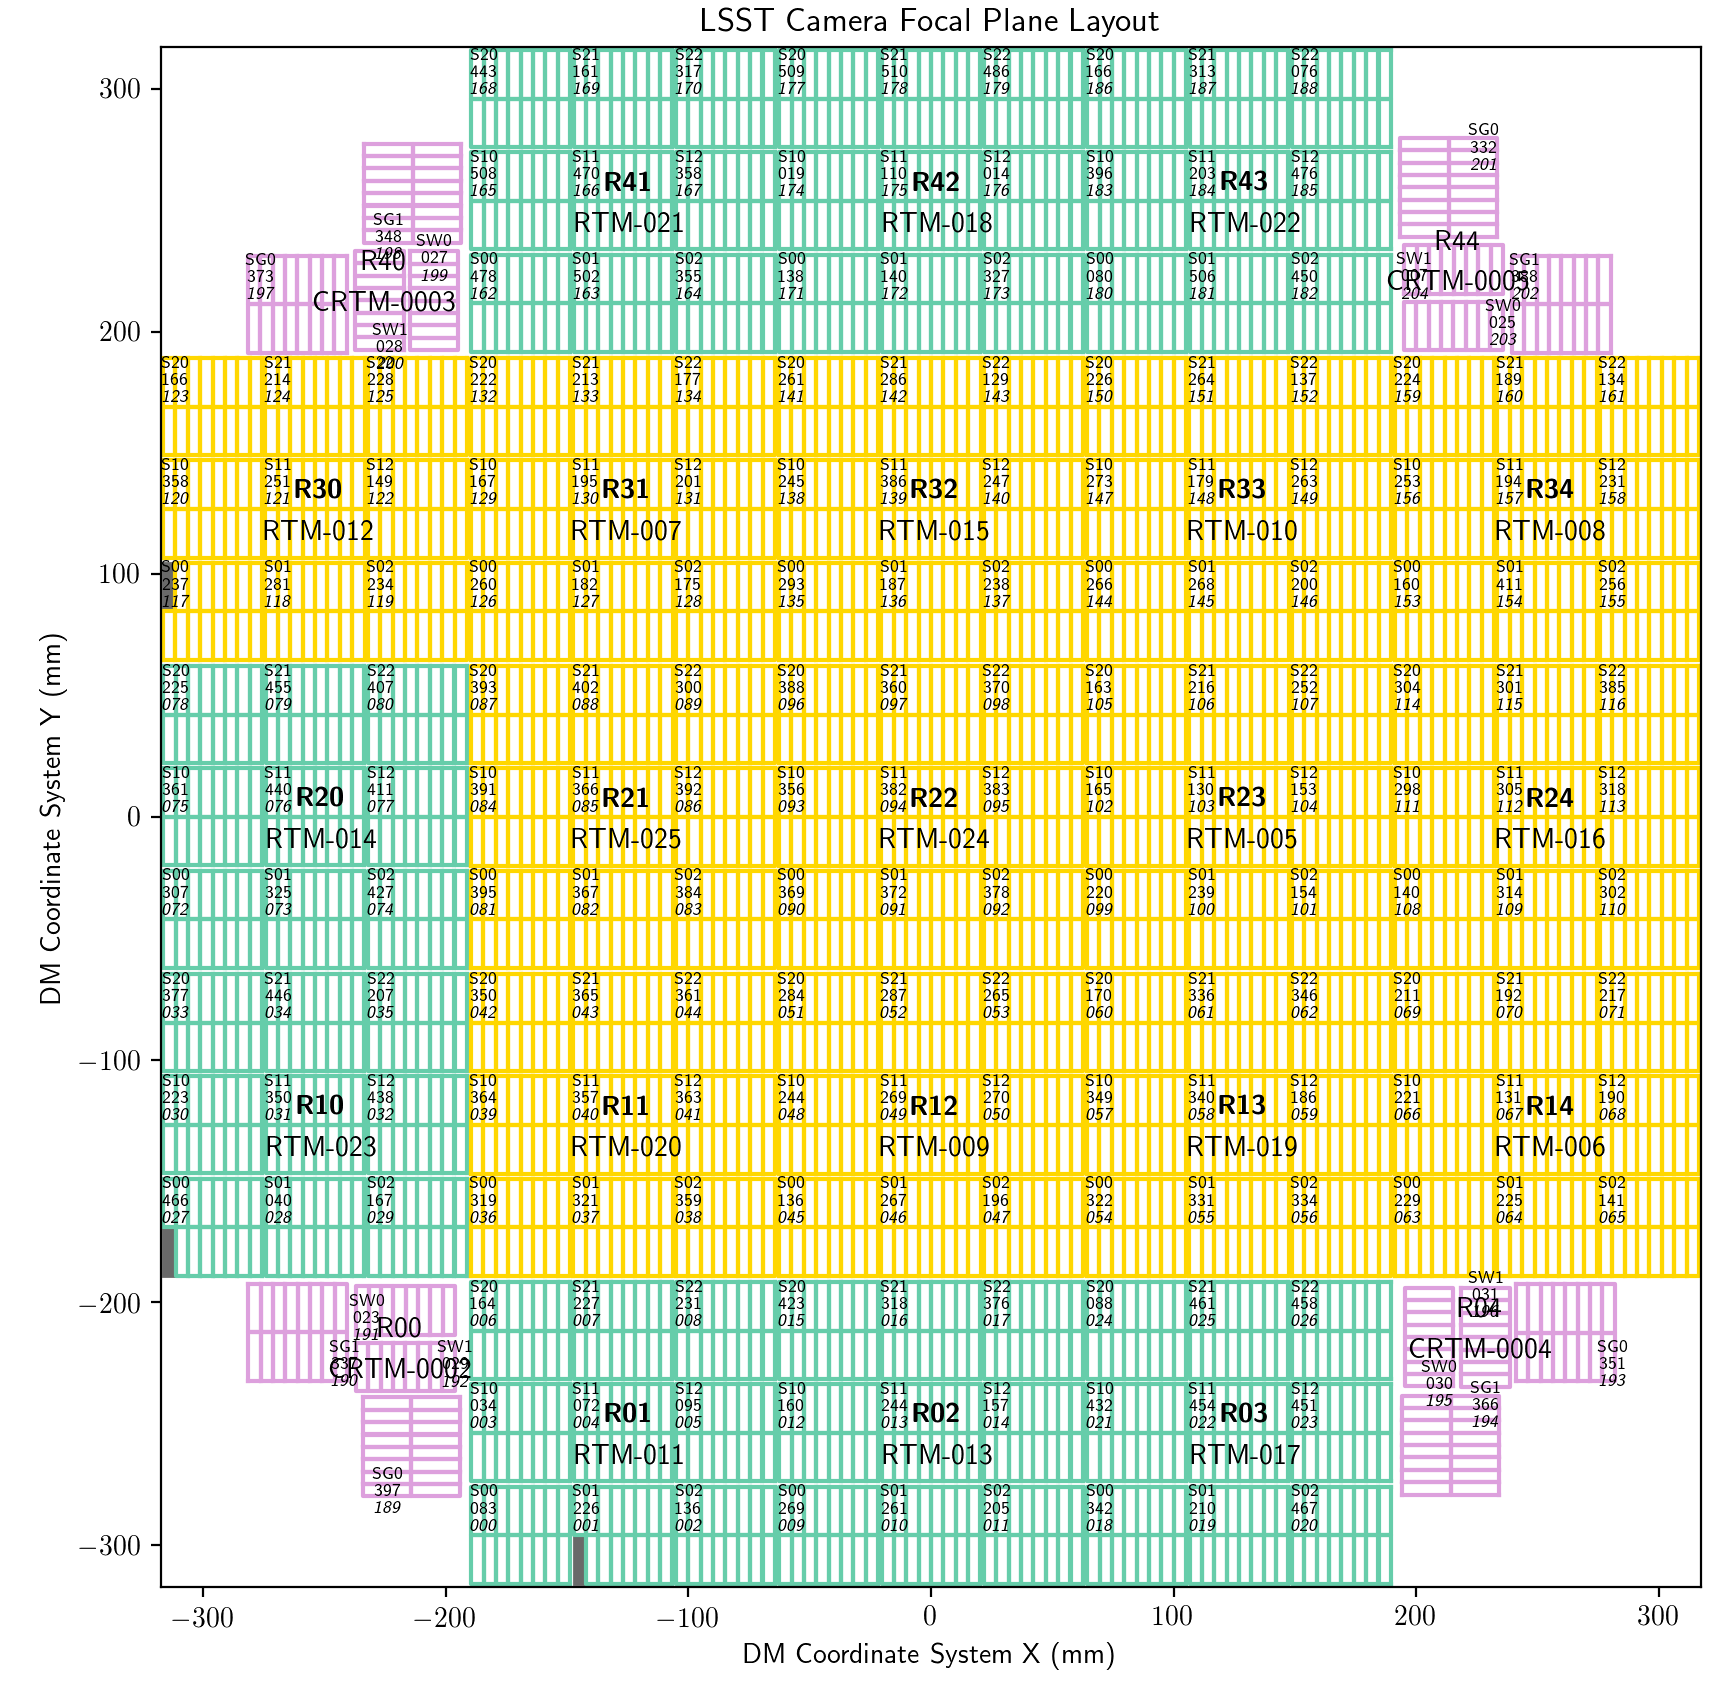
\includegraphics[width=\textwidth]{Figures/FP_layout_DM.png}
%    \caption{The focal plane of the LSST camera. The vendor's CCDs' location is blue for ITL and yellow for E2V. Each CCD (a small square) is composed of 16 segments, each with its amplifier, and 189 CCDs are responsible for taking the science data. The CCDs at the corners are for focusing and synchronization with the Earth's rotation (see \href{https://www6.slac.stanford.edu/news/2020-09-08-sensors-world-largest-digital-camera-snap-first-3200-megapixel-images-slac.aspx}{LSST-SLACLab})}
%    \label{fig:FP_LSSTCam}
%\end{figure}
%
%\subsection{What is Photon Transfer Curve (PTC)?}
%
%The Photon Transfer Curve (PTC) allows the characterization of the fundamental parameters of the CCD, mainly the determination of the relationship between the electrons recorded by each pixel and their conversion to analog-to-digital counts (ADU), i.e., the gain; it also measures the nonlinearity of the camera and its Full Well Capacity (FWC). The first parameter is essential because other vital parameters, such as read noise, quantum efficiency, dark current, among others, depend on it \citep{downing2006ccd}.
%
%Figure \ref{fig:PTC} shows the PTC of segment C06 of sensor 22 of the LSSTCam, where it is evident that at low fluxes, the variance is low and increases with the flux but not linearly until the saturation point or FWC, which for this detector is $83000$ ADU. After this point, the variance begins to decrease, indicating that the flux stored in each pixel of this amplifier begins to homogenize. The nonlinear behavior of this curve is exhibited by \textit{thick fully-depleted CCDs}, according to \cite{downing2006ccd} charge storage in a pixel is the main reason, since the expected relationship between the variance and the mean number of counts in a pixel is modified in flat images \citep{walter2015brighter}. The effective area of the pixel changes with the amount of charge, decreasing the more significant the charge accumulated in the pixel. Consequently, very bright sources are mainly affected by this so-called BF effect. If the pixels of the CCD segment were independent, they could be described by Poisson statistics, and the PTC would follow the green line in the figure.
%
%\begin{figure}[!htb]
%    \centering
%    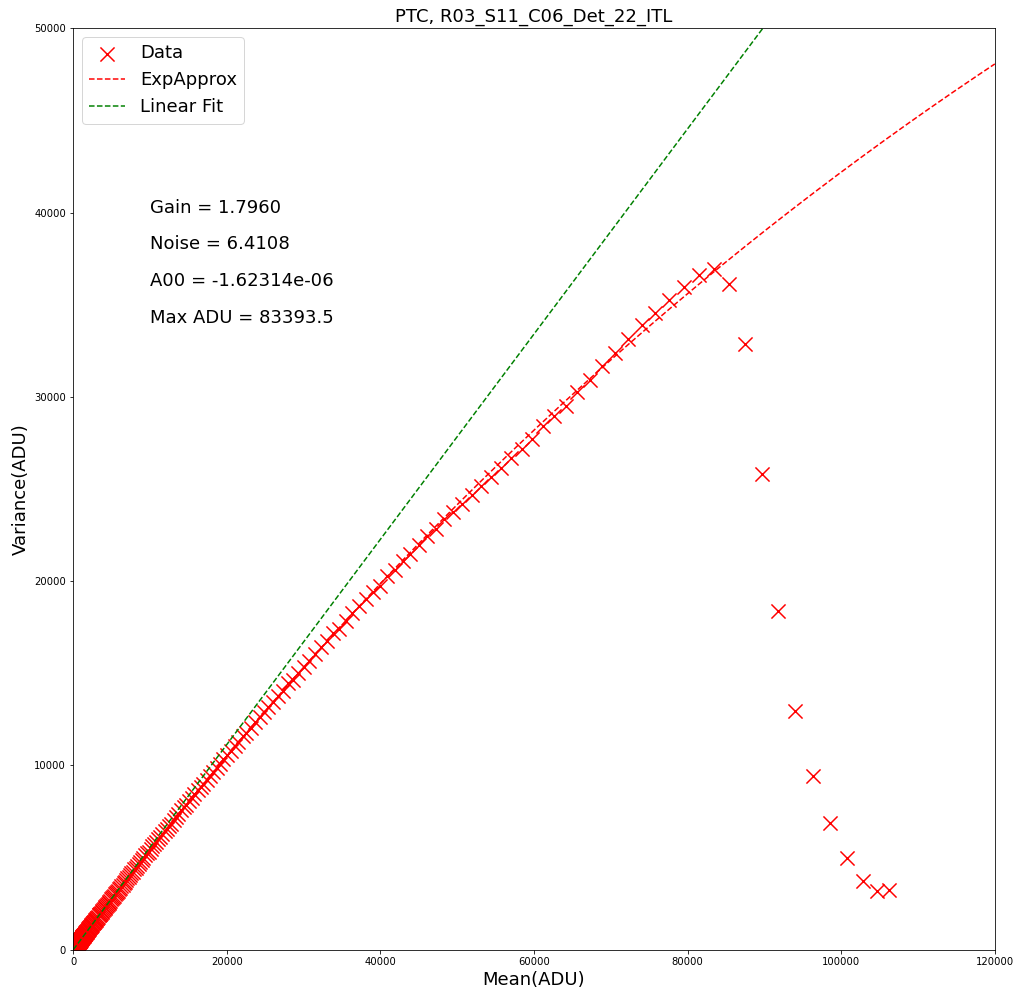
\includegraphics[width=0.7\textwidth]{Figures/PTC_R03_S11_C06_Det22.png}
%    \caption{PTC for detector 22 was found in raft 03, sensor 11, and amplifier C06; its vendor is ITL. In red crosses, the data are shown, the red line uses the EXPAPPROXIMATION fit, and the green line is a linear fit. This curve was constructed with the results obtained via \textit{DM stack}.}
%    \label{fig:PTC}
%\end{figure}
%
%\subsubsection{Brigther father effect}
%
%As mentioned above, the charge stored in a pixel modifies the effective area of the pixel, decreasing the probability that this pixel will continue to store the charge. Consequently, the electrons that should have been kept in this pixel are deflected horizontally, causing more elliptical images. Thus, a process initially described by a Poisson statistic, and the charge stored in each pixel was independent of the other, breaks down by modifying the relationship between the variance and the mean number of counts per pixel \citep{walter2015brighter}. This effect changes the PSF, so it is a potential problem in surveys interested in the variation of the brightness and shape of objects \citep{coulton2018exploring}
%
%
%\vspace{6mm}
%
%
%This work was developed during the RECA (Red de Estudiantes Colombiana de Astronomía) internship program 2022\footnote{RECA internship program is a training program in scientific research in Astronomy, Astrophysics, and Cosmology directed to students of Colombian institutions. The program website \href{https://recastronomia.github.io/internship/}{https://recastronomia.github.io/internship/}}. The program was carried out over three months, in which we also developed other activities such as remote astronomical observations with the Teide Observatory\footnote{\href{https://www.iac.es/es/observatorios-de-canarias/observatorio-del-teide}{https://www.iac.es/es/observatorios-de-canarias/observatorio-del-teide}}.
%
%
%In this report, we present the data used in the section \ref{sec:data}. The section \ref{sec:methods} describes the methodology used. In the section \ref{sec:results}, we present the results and analysis. Finally, the conclusion in section\ref{sec:conclusions}.
\section{Data} \label{sec:data}
The data used in this study were obtained using the Bench for Optical Testing (BOT), which was constructed and designed at SLAC National Accelerator Laboratory. The BOT enables laboratory tests with the LSSTCam, ensuring that flat images exhibit variations of less than 5\% for accurate measurements of linearity, FWC, and gain from the PTCs \citep{newbry2018lsst}. Figure \ref{fig:BOT_stand} illustrates the structure of the BOT, with the cryostat located at the circular top and the focal plane pointing downwards on the test bench.

\begin{figure}[!htb]
    \centering
    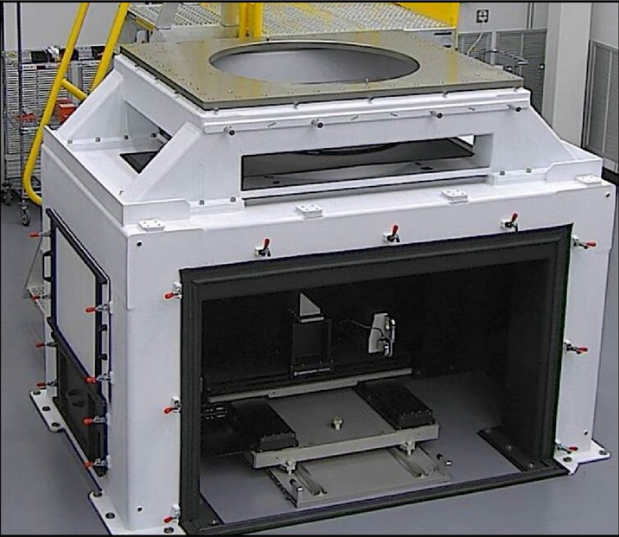
\includegraphics[width=0.7\textwidth]{Figures/BOT_stand.png}
    \caption{Bench for Optical Testing (BOT) designed by SLAC. Figure is taken from \cite{newbry2018lsst}. }
    \label{fig:BOT_stand}
\end{figure}

The data for this study were obtained from \textit{run 13144} and \textit{run 13186}, with the latter containing the crosstalk matrix information. As described in \cite{snyder2020laboratory}, electronic crosstalk measurements were conducted using a projector known as the \textit{crosstalk projector}, which illuminates a single sensor with a collimated beam of light with a pattern containing large bright spots, each with a radius of 80 pixels. However, for laboratory tests simulating realistic source sizes, the \textit{spot grid projector}, an optical projector, was used. This projector generates spots in specific grids and includes filters to simulate both satellite trails and the signal level of the sky background.
%\section{Methodology} \label{sec:methods}

The images used in this study underwent standard reduction techniques, including overscan, bias, dark, and defects reduction. Defects reduction involves creating maps that indicate regions with both bright and dark defects, such as dead pixels. These reductions serve as the starting state for the PTC study. Subsequently, other corrections, such as linearity and crosstalk, are applied to analyze their effects on the main parameters of the camera.

\vspace{3mm}
Professor Craig Lage generated supercalibrations for the entire focal plane, which are stored in his personal collection at \textit{u/cslage/calib/13144/calib.20220103}. The images shown in Figures \ref{fig:superbias} and \ref{fig:superdark} are superbias and superdarks, respectively, generated as part of the learning process for producing the calibration images using the LSST's software called \textit{DM stack}.

\vspace{3mm}
The code used to generate the calibration images via \textit{DM stack} can be found at \href{https://github.com/lsst/cp_pipe}{https://github.com/lsst/cp\_pipe}. This code generates the data for the construction of the PTC and calculates the gain for each CCD segment as its FWC. Additionally, it calculates the gain using another method, which was analyzed in Section \ref{subsec: method_gainflat} to determine the differences between it and the PTC method. The alternative method involves using two pairs of flats for gain estimation. We utilized two versions of the \textit{DM stack} code\footnote{The DM stack software is developed for the LSST and is publicly available on GitHub at \href{https://github.com/lsst/}{https://github.com/lsst/}} for the entire focal plane:

\begin{itemize}
    \item w\_2022\_27: Initial version we started working with.
    \item w\_20222\_32: Version that includes one of our main results on obtaining the gain with pairs of flats (see the \href{https://jira.lsstcorp.org/browse/DM-35790}{DM-35790} ticket in Jira).
\end{itemize}
%\section{Results} \label{sec:results}


\subsection{Photon Transfer Curve}

As part of this project, a key initial task was to utilize the PTC to determine essential parameters for each CCD segment across the focal plane using the \textit{DM stack}. This has already been done by SLAC National Accelerator Laboratory\footnote{The code used by SLAC is available at \href{https://github.com/lsst-camera-dh/eotest/blob/32c17b0a33b9c099651ed581ee90c1b1101012fb/python/lsst/eotest/sensor/ptcTask.py}{SLAC code}} (referred to as SLAC hereafter) for this particular run (\href{https://srs.slac.stanford.edu/BOT_EO_Reports/13144/}{SLAC heat maps BOT 13144}), and we aim to reproduce their results in this study.

\vspace{3mm}

%%%%%%%%%%%%Figura

\begin{figure}[!htb]
    \centering
    \includegraphics[width=\textwidth]{Figures/PTC_Detector55.png}
    \caption{PTC for all segments of sensor 55 (E2V). The Xs represent the data points, the red line is the exponential fit to the PTC using the Astier16 approximation (eq. \ref{eq:Astier16}), and the green line is a linear fit. The obtained fit parameters include the gain, the $a_{00}$ parameter, the PTC turnoff (Max ADU), and the read noise.}
    \label{fig:PTC_55}
\end{figure}

%%%%%%%%%%%%%%%%%%

Initially, PTCs were generated by CCD for the entire focal plane, as shown in Figure \ref{fig:PTC_55}, to detect any abnormal behavior and low PTC-turnoff values (below 40000 ADU). Detectors found with low PTC-turnoff and/or misclassified were recorded in Table \ref{tab:PTC_warnings}. Furthermore, a visual inspection revealed that approximately 60 \% of the detectors had at least one segment exhibiting a \textit{Downing dip}.

\vspace{3mm}
%%%%%%%%%%%%Figura

\begin{figure}[!htb]
 \centering
     \begin{subfigure}[b]{0.49\textwidth}
         \centering
         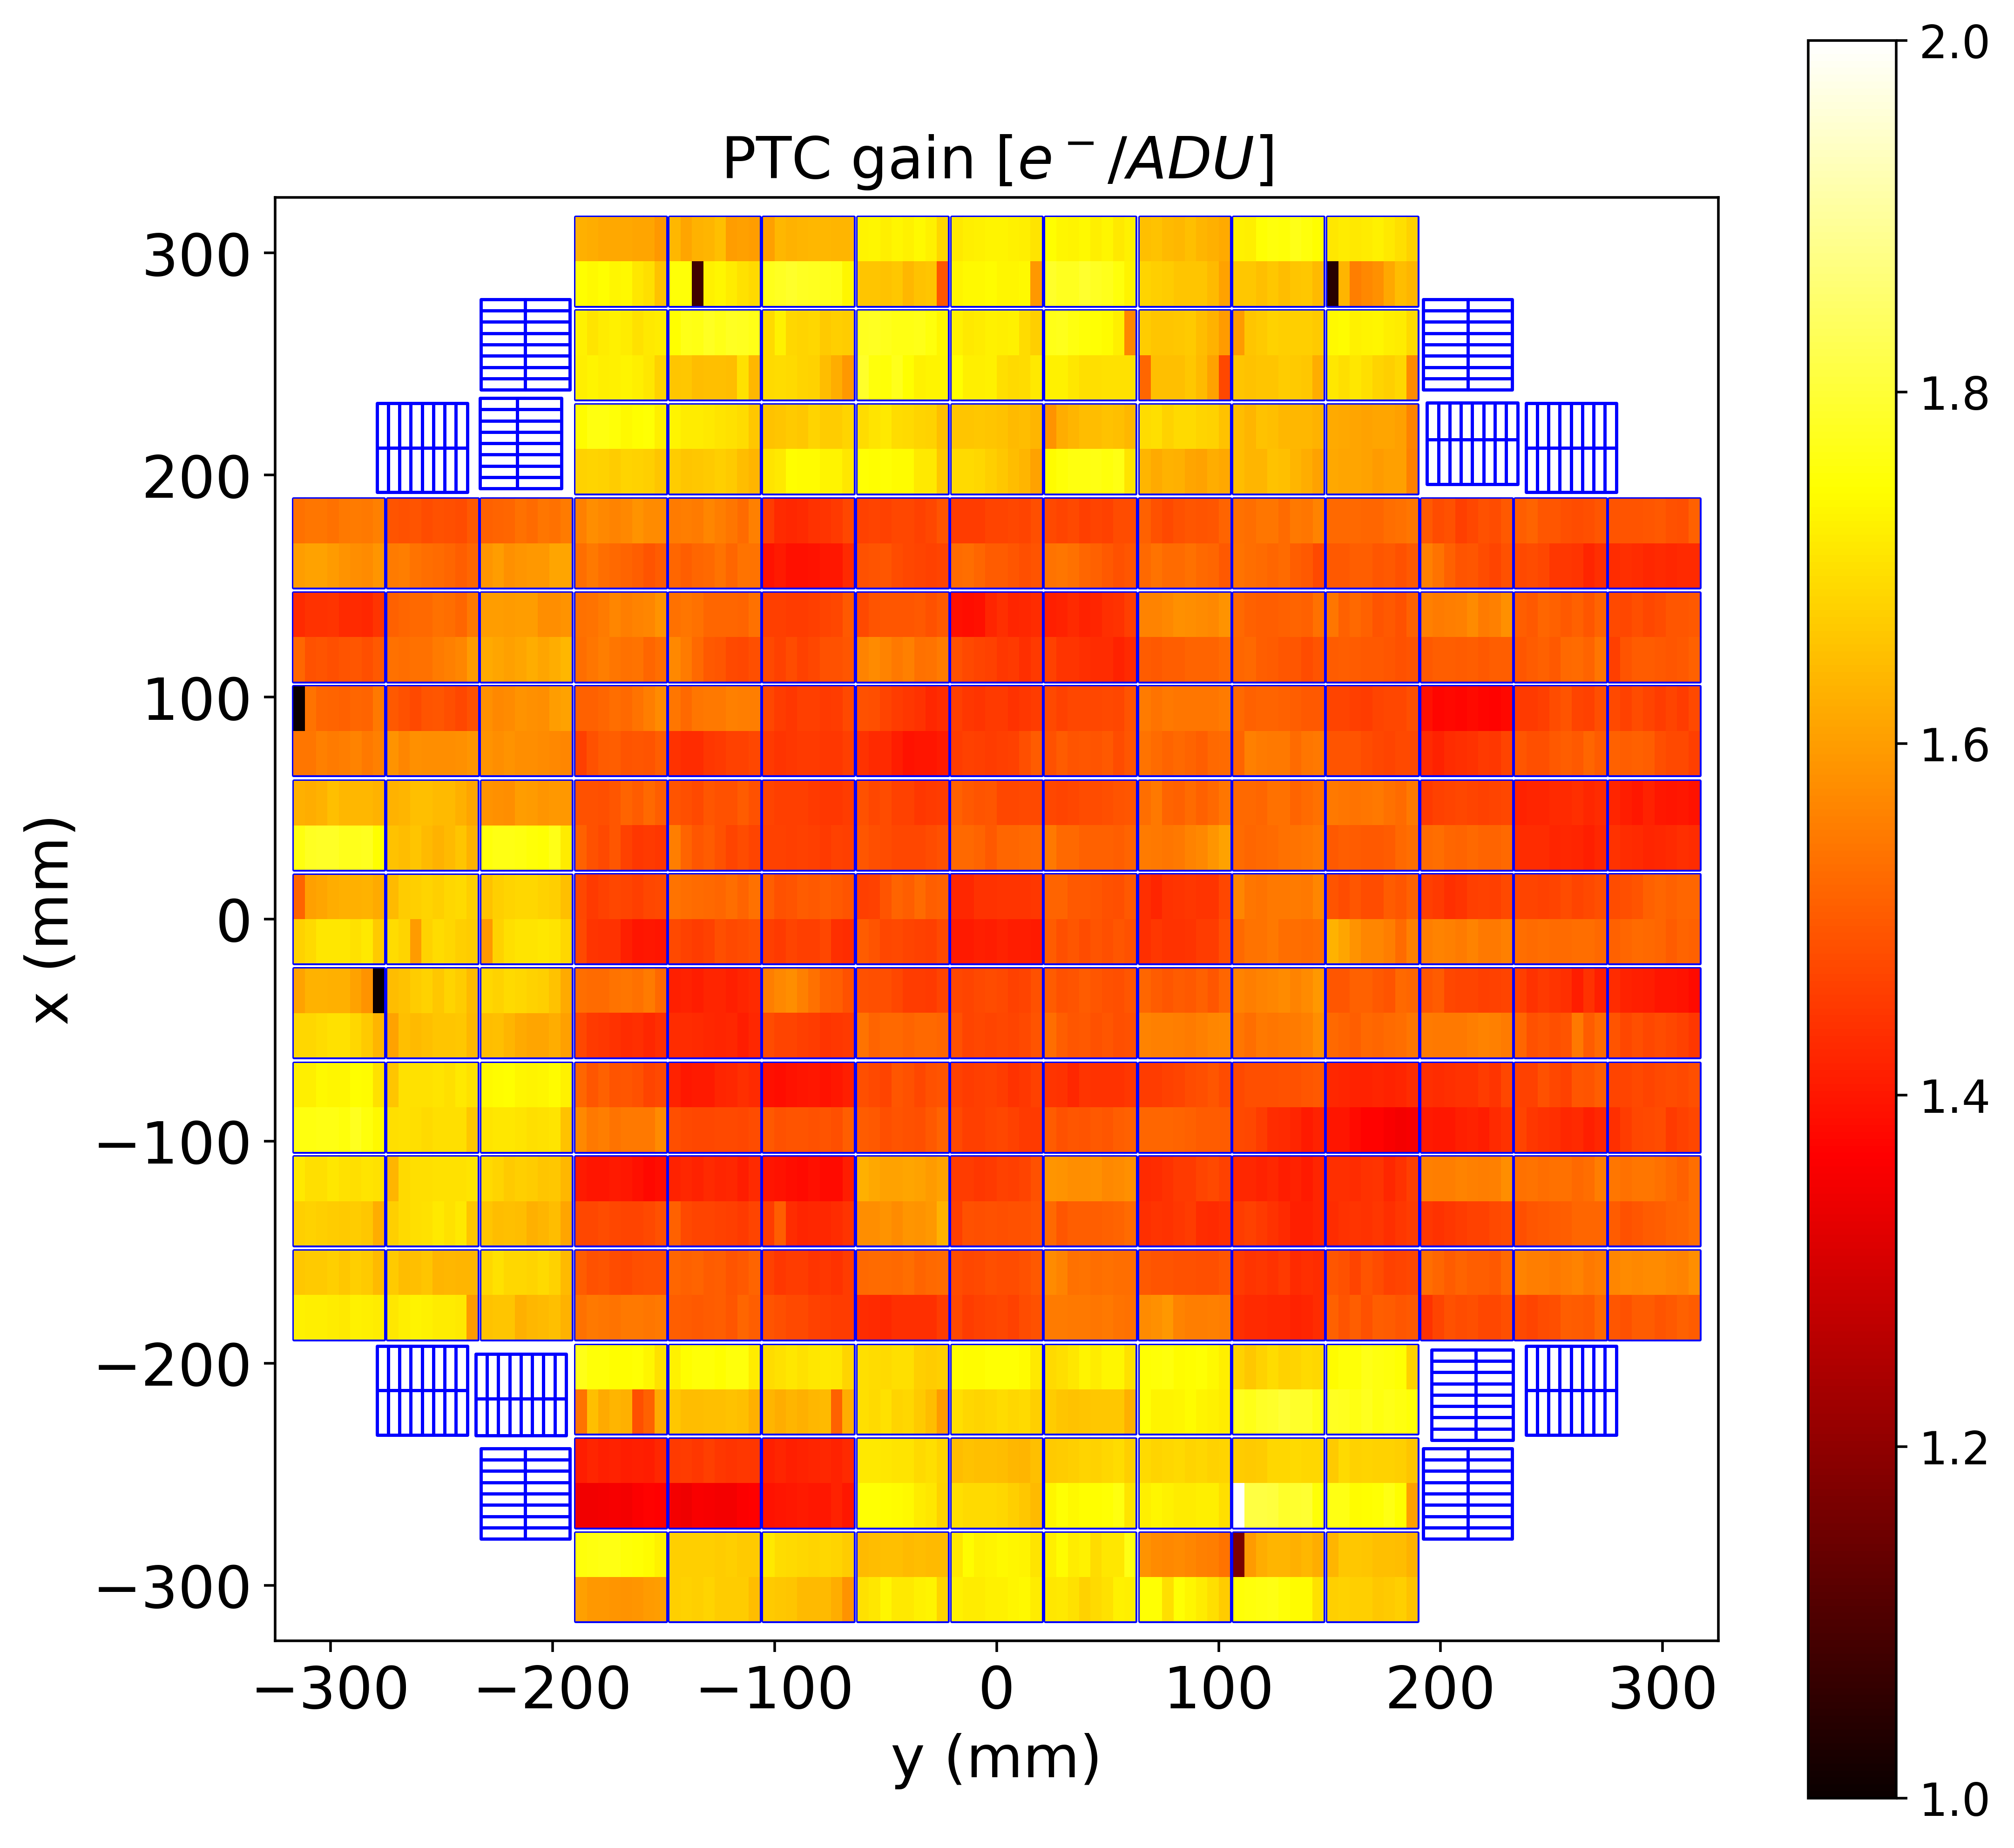
\includegraphics[width=\textwidth]{Figures/Focal_plane_gain.png}
     \end{subfigure}
     \hfill %\hspace{-10em}
     \begin{subfigure}[b]{0.49\textwidth}
         \centering
         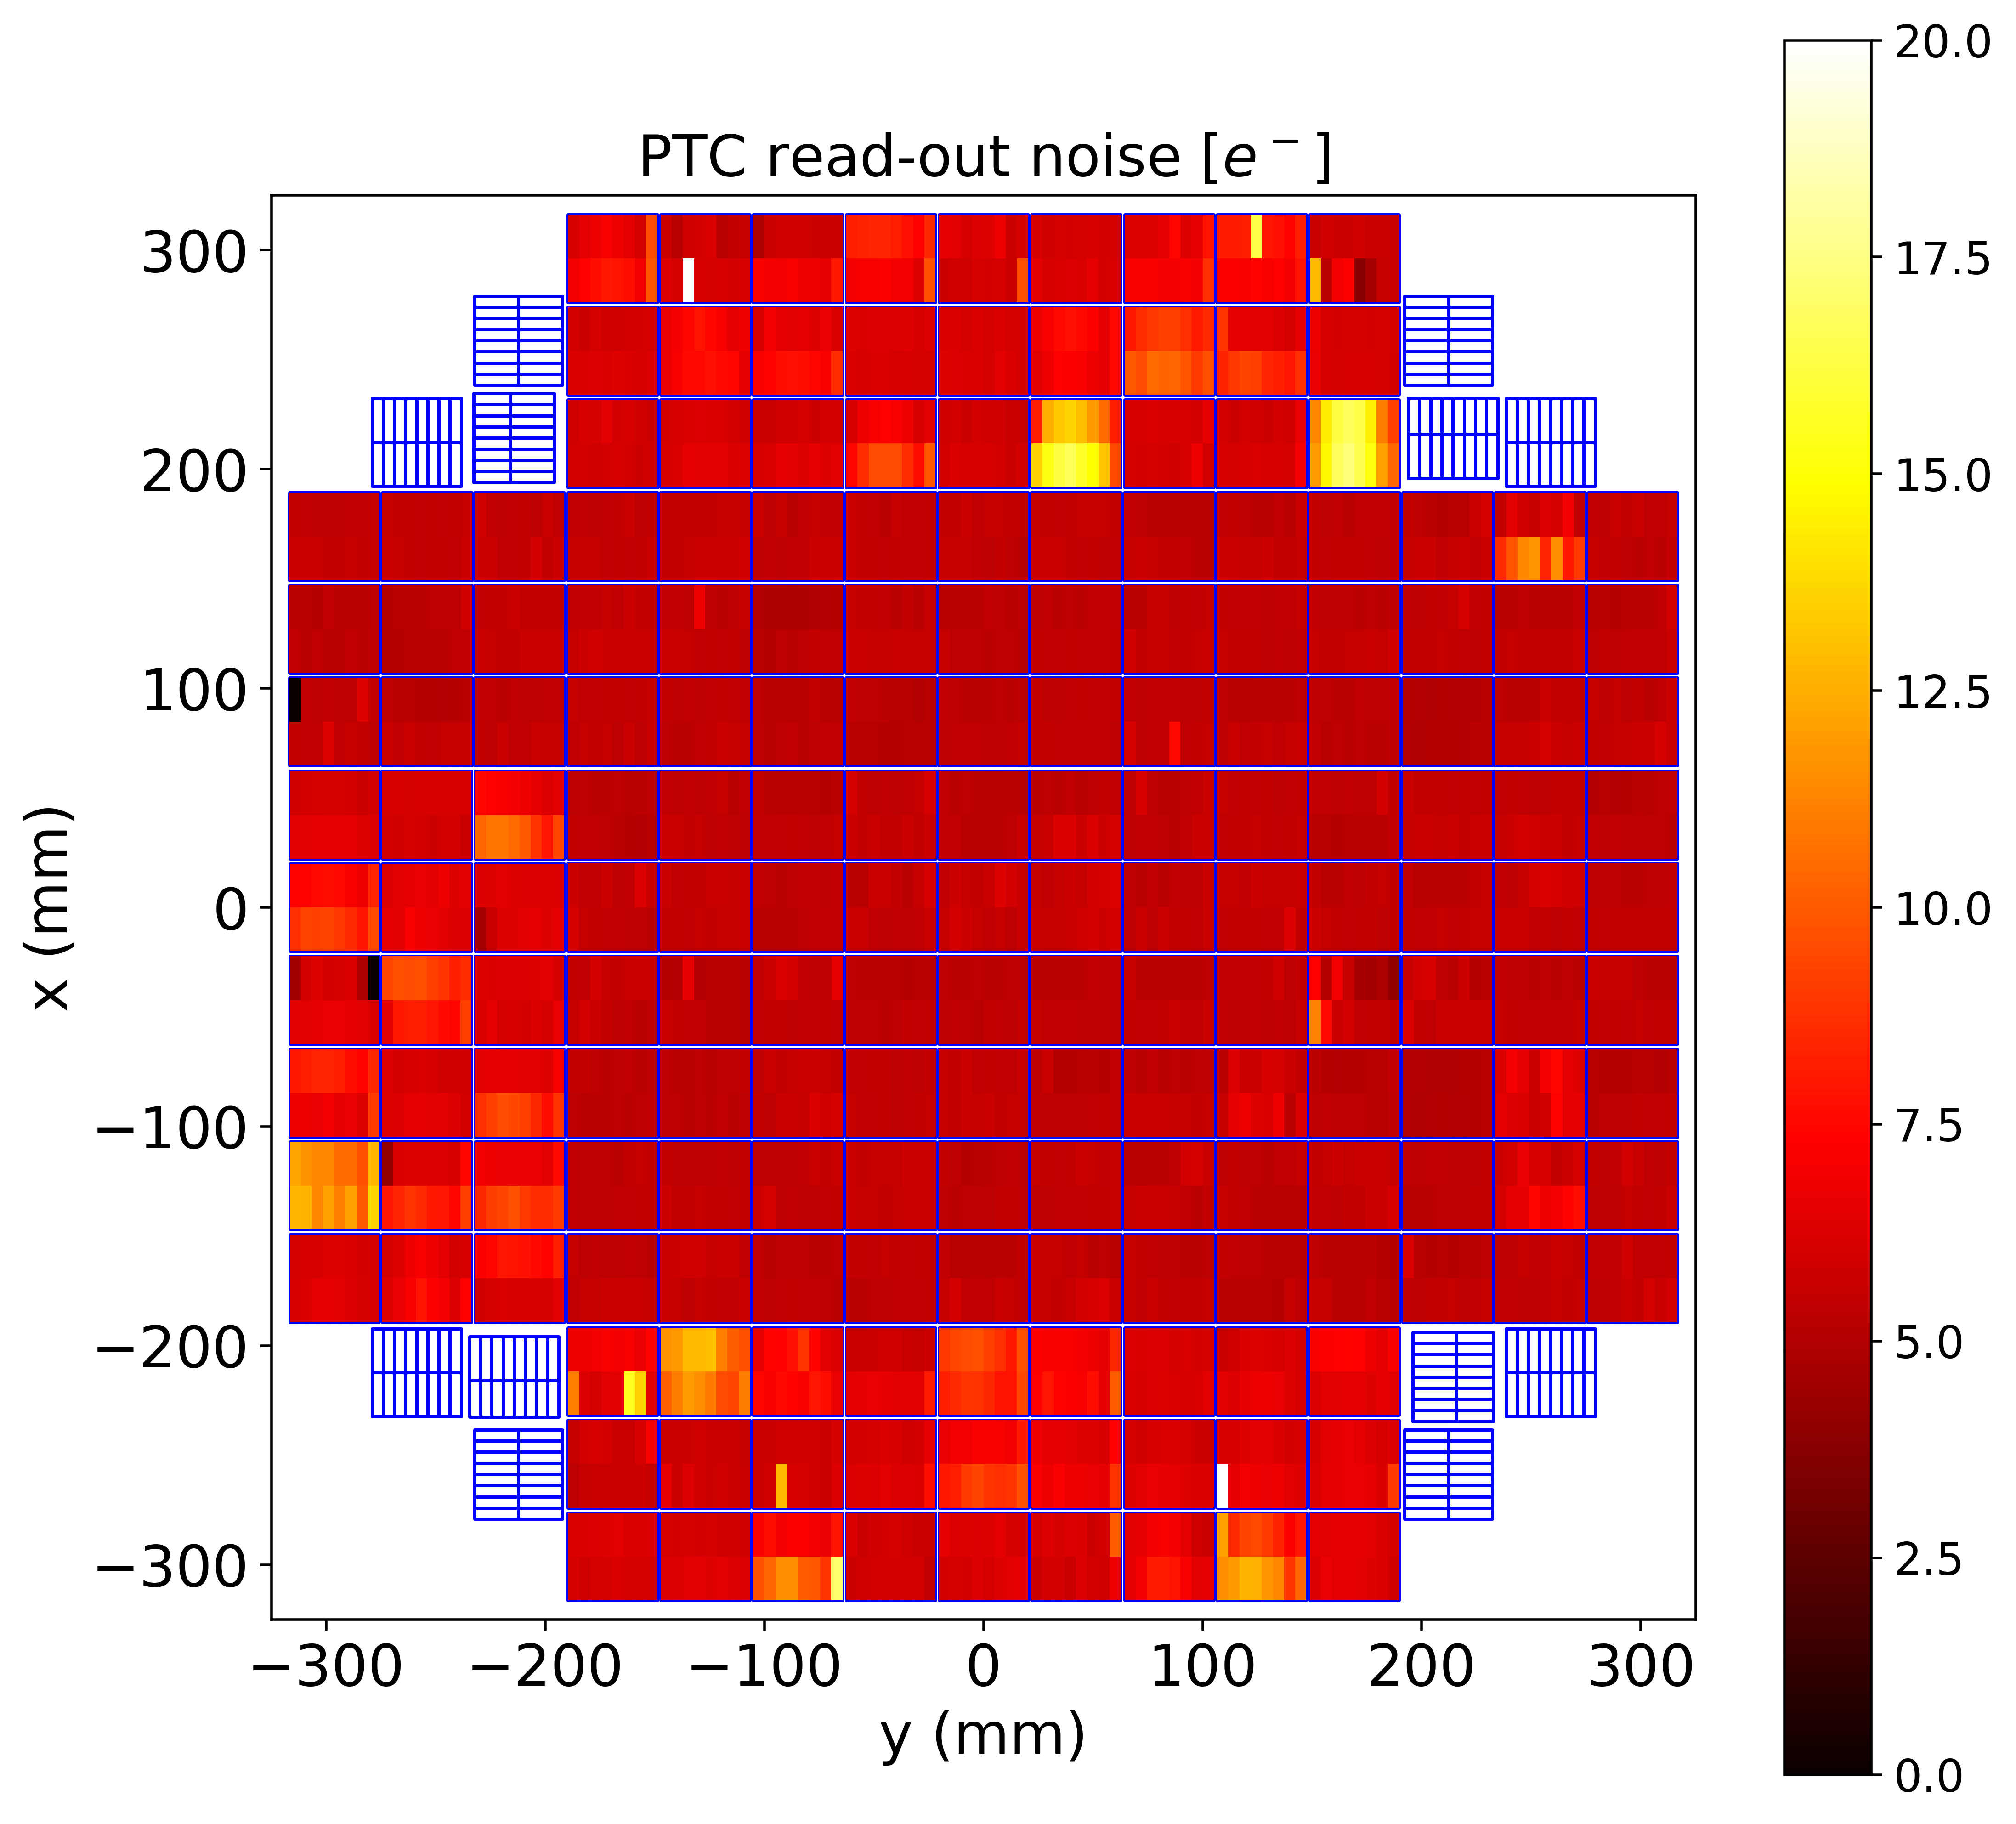
\includegraphics[width=\textwidth]{Figures/Focal_plane_noise.png}
     \end{subfigure}
     \vspace{3mm}
     \begin{subfigure}[b]{0.49\textwidth}
         \centering
         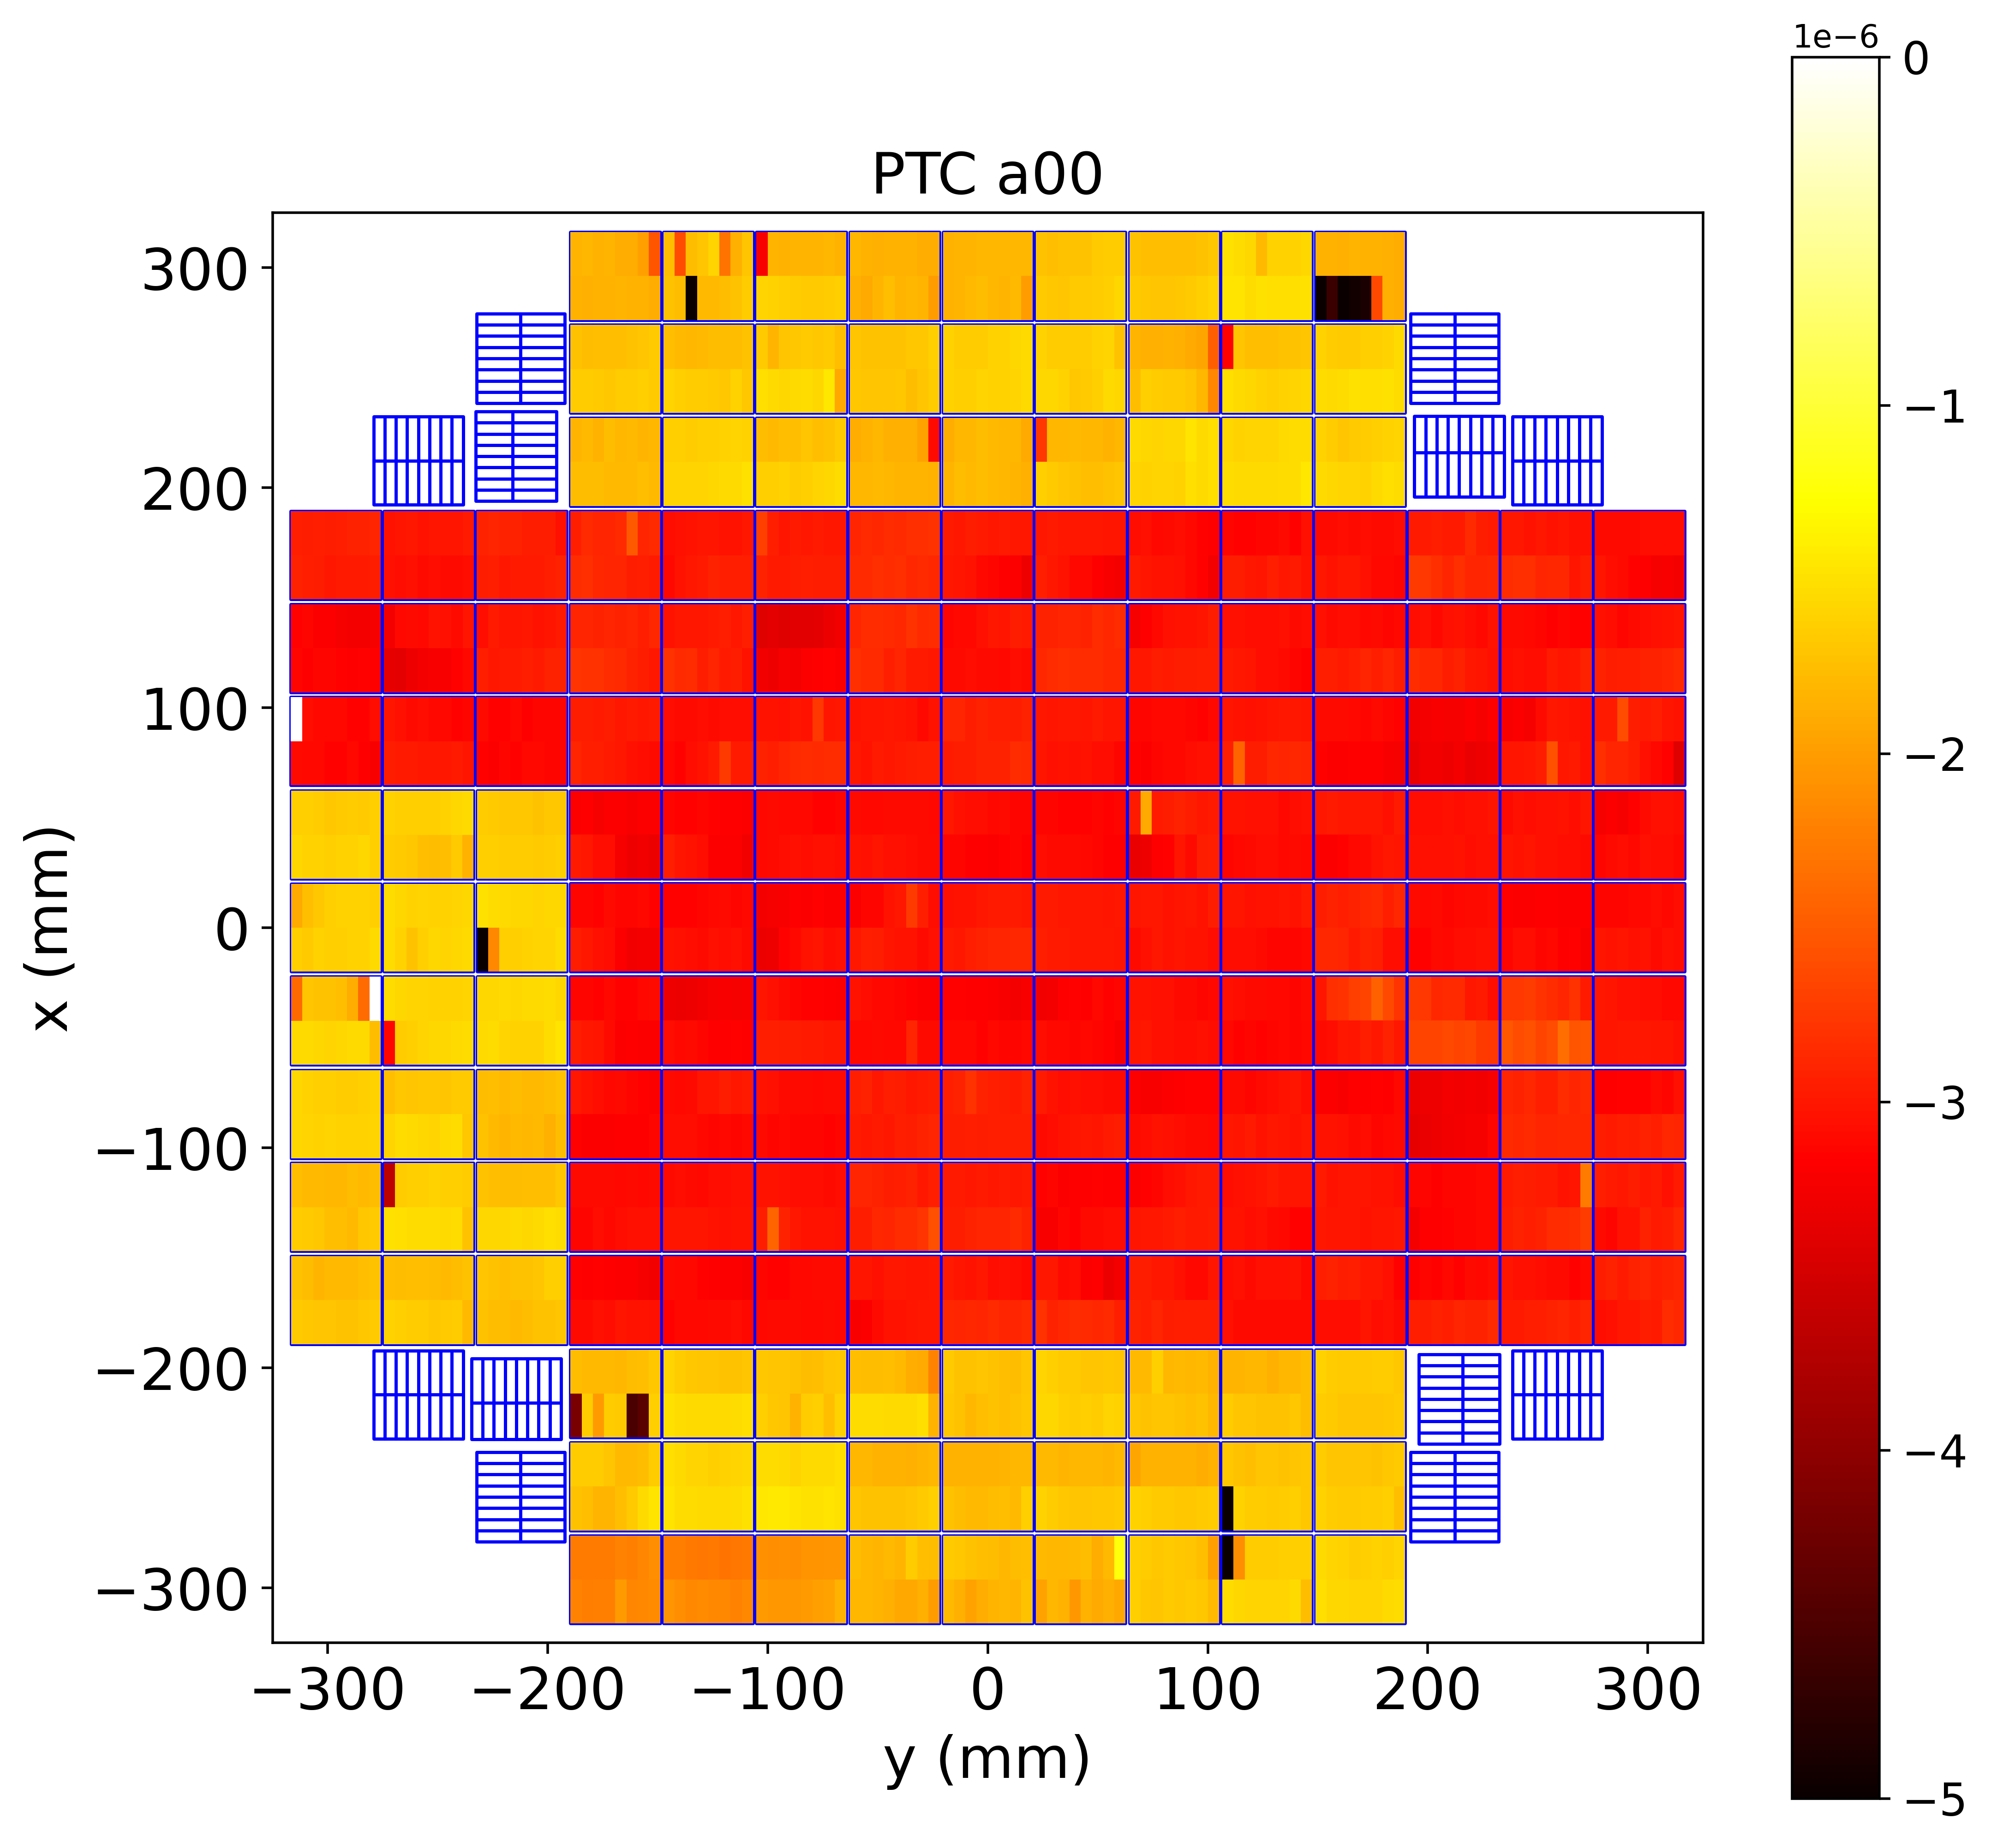
\includegraphics[width=\textwidth]{Figures/Focal_plane_a00.png}
     \end{subfigure}    
     \hfill
     \begin{subfigure}[b]{0.49\textwidth}
         \centering
         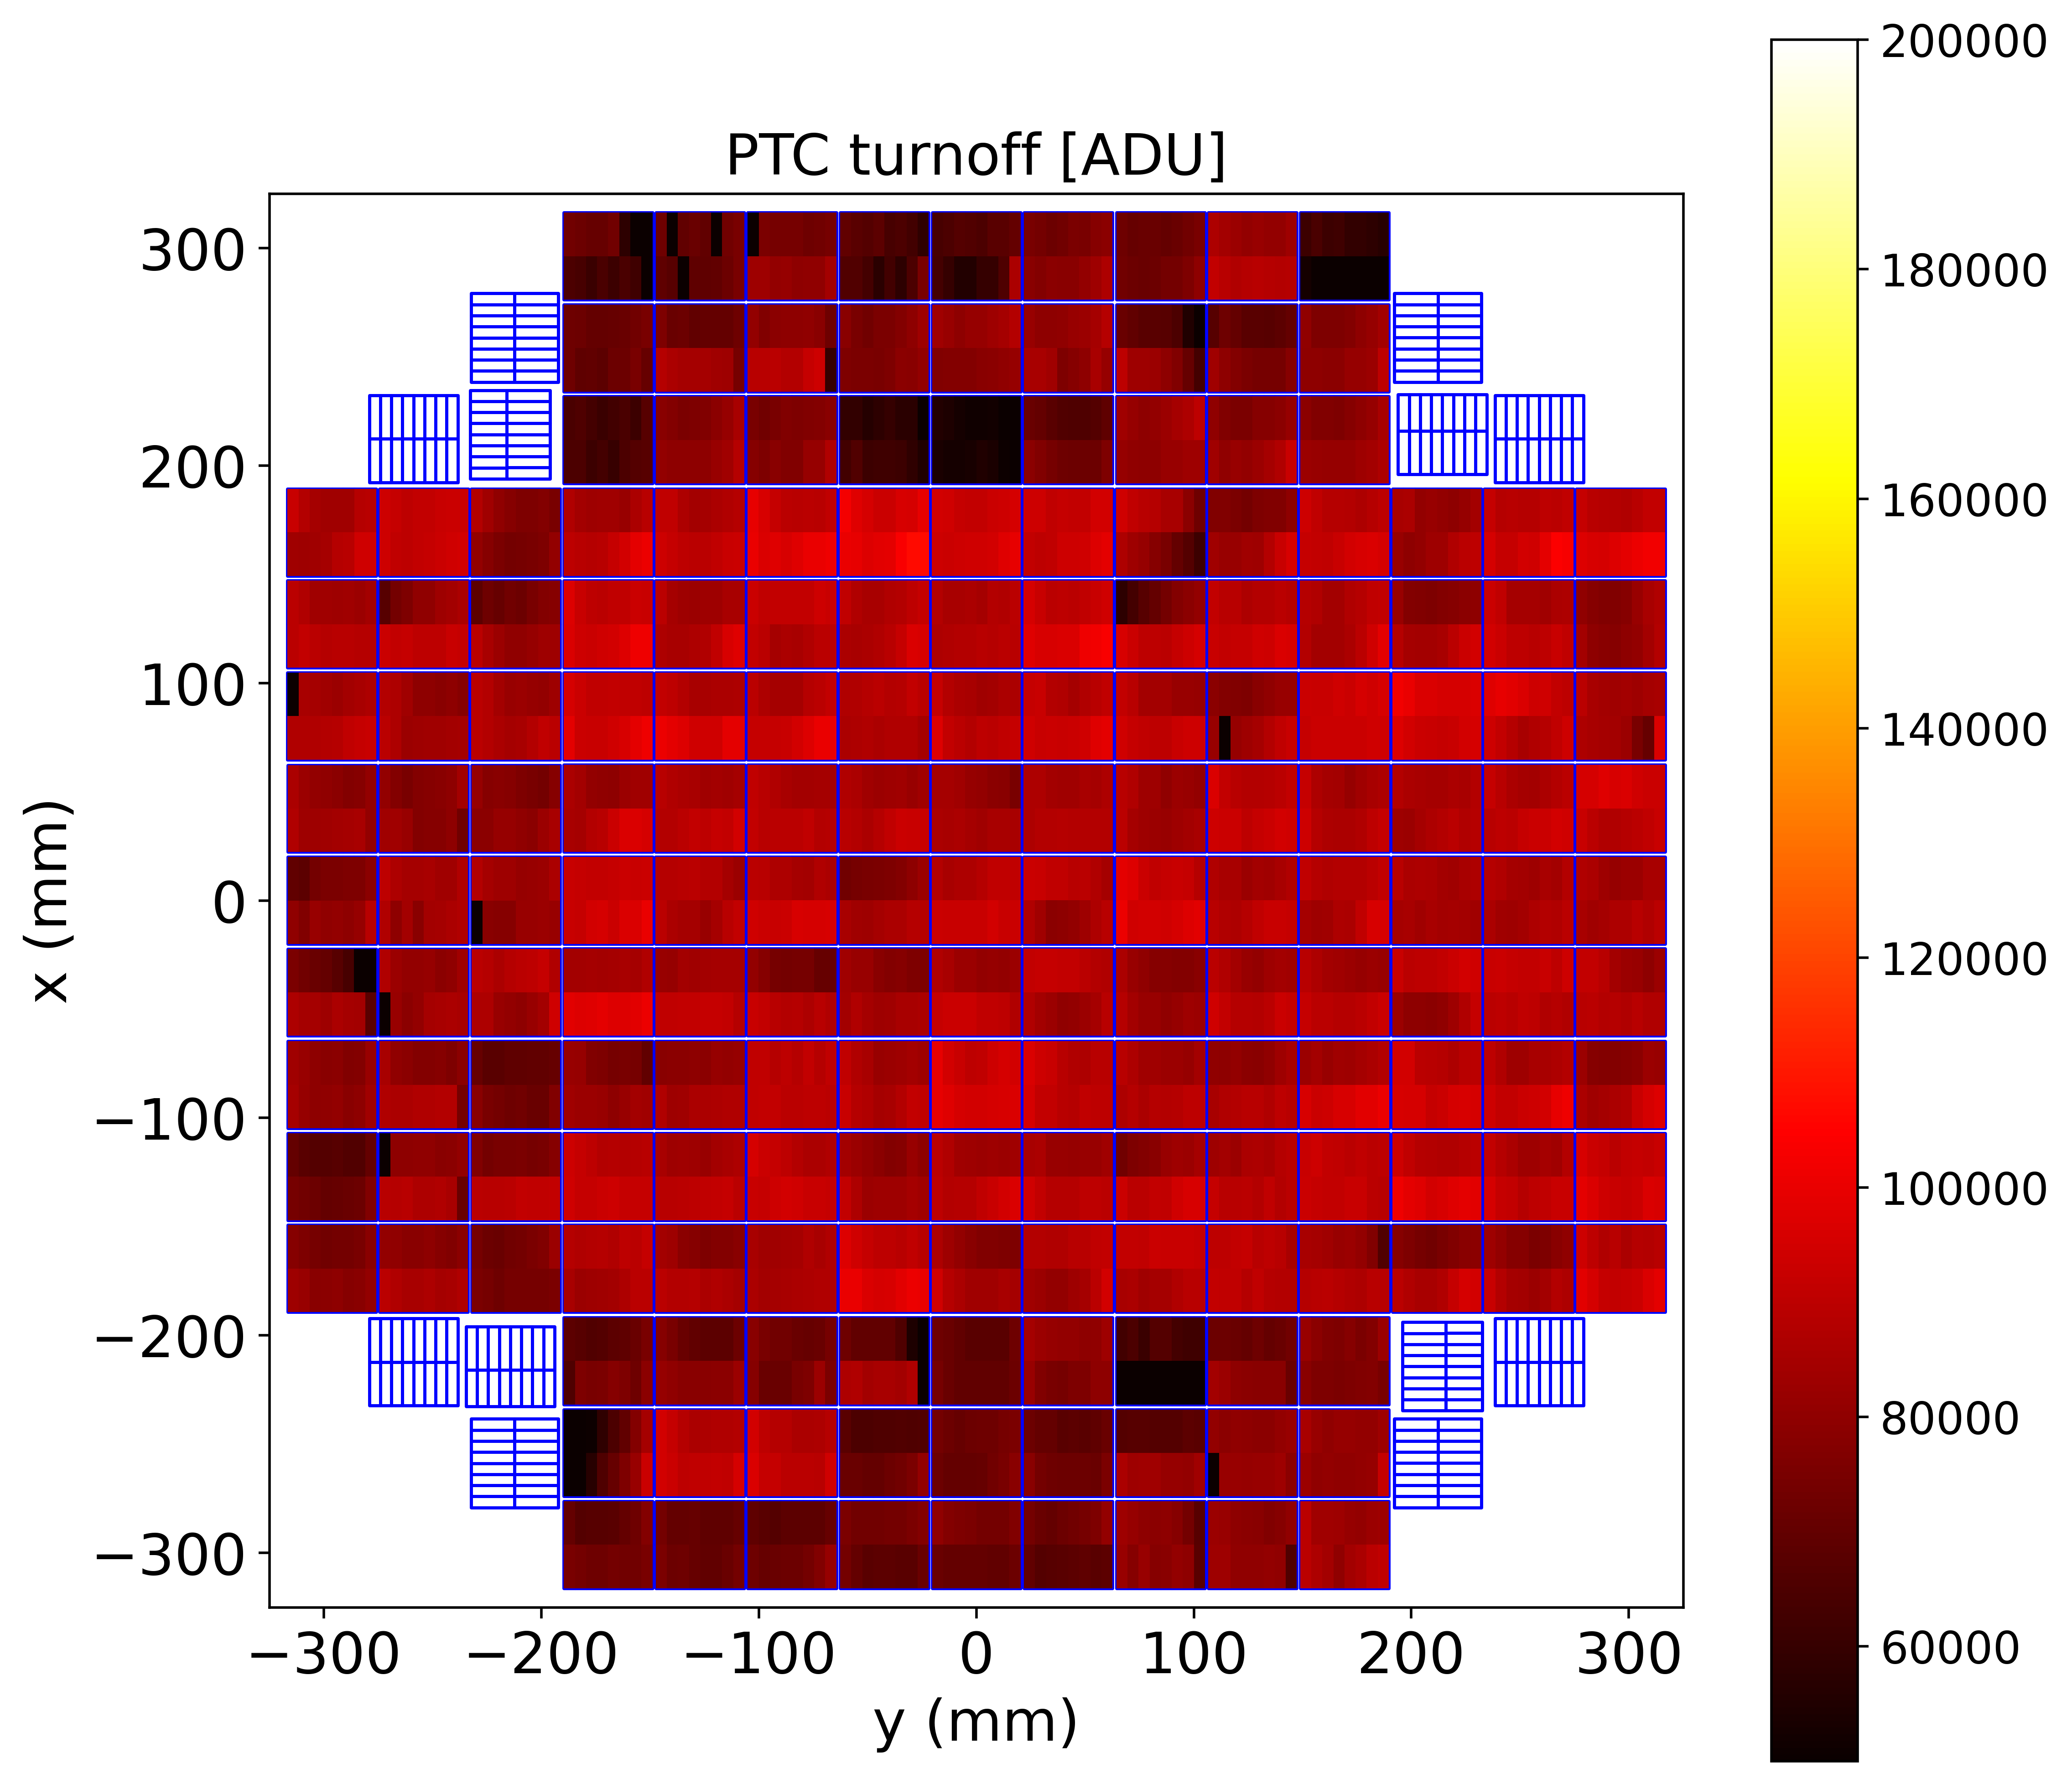
\includegraphics[width=\textwidth]{Figures/Focal_plane_turnoff.png}
     \end{subfigure}
        \caption{Heatmaps depicting the parameters obtained by fitting the PTC for each segment of the sensors across the entire focal plane. The upper panel shows the gain values on the left and the read noise on the right. The lower panel shows the values of $a_{00}$, which are of the order of $-1 \times 10 ^{-6}$, on the left, and the turnoff on the right. These maps are a reproduction of those previously constructed by SLAC for the same run 13144 (\href{https://srs.slac.stanford.edu/BOT_EO_Reports/13144/}{SLAC heat maps}.}
        \label{fig:FocalPlane_PTC}
\end{figure}
%%%%%%%%%%%%%%%%%%
Subsequently, heat maps were generated for the entire focal plane, similar to those performed by SLAC, as shown in the panels of Figure \ref{fig:FocalPlane_PTC}, to visualize the parameters estimated by fitting the PTC: gain and read noise in the upper left and right panels, respectively, and $a_{00}$ and turnoff in the lower left and right panels, respectively. Notably, bimodality is observed in the gain and $a_{00}$ values, which account for the BF effect. The more reddish values dominate in the E2V sensors, while the more yellow values dominate in ITL sensors, indicating that E2V vendor's detectors generally have a lower gain but more negative BF effect coefficients compared to ITL. In contrast, no significant effect is exhibited due to the vendor for readout noise and turnoff.

\vspace{3mm}
The histograms in Figure \ref{fig:Histogram_PTC} support the behavior described above by the heat maps, revealing clear bimodality for gain and $a_{00}$, and a more generalized behavior for read noise and turnoff. The average gain values for E2V sensors are $1.49 \pm 0.05$ $e^{-}/ADU$, and for ITL sensors are $1.69 \pm 0.05$ $e^{-}/ADU$. The average BF effect coefficient values are $(-3.0 \pm 0.1)\times 10 ^{-6}$ for E2V and $(-1.7 \pm 0.2)\times 10 ^{-6}$ for ITL.

\vspace{3mm}

%%%%%%%%%%%%Figura
\begin{figure}[!htb]
    \centering
    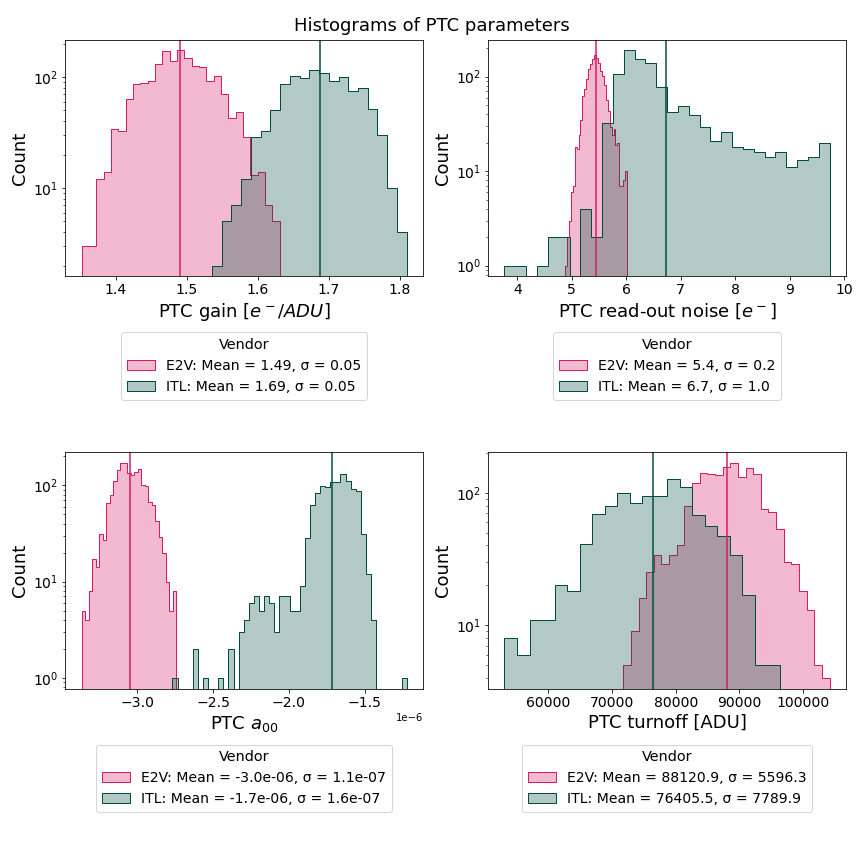
\includegraphics[width=\textwidth]{Figures/Histograms_PTC.png}
    \caption{Histograms showing the distribution of parameters obtained from the fit to the PTC: gain (top left), read noise (top right), $a_{00}$ (bottom left), and turnoff (bottom right). The distributions are shown separately for each vendor, with magenta representing E2V and blue representing ITL. The vertical lines indicate the mean value of each distribution.}
    \label{fig:Histogram_PTC}
\end{figure}

%%%%%%%%%%%%%%%%%%
Although the results of this work are generally congruent with those obtained by SLAC, some differences were found in certain segments, particularly for gain values in segments C04 and C14 of detector 0 (R01\_S00), C00 of detector 22 (R03\_S11), and C02 of detector 169 (R41\_S21). Table \ref{tab:PTC_warnings} highlights these segments in red, where the most notable differences between our results and those of SLAC were observed for the four parameters (gain, BF coefficient, read noise, and turnoff). For detector 22, the values on the table suggest that the detector may possibly be dead, while for the segment of detector 169, there may be a misclassification by the PTC-turnoff location algorithm. These specific cases could be the reason for the differences between our results and those of SLAC. However, to determine the precise cause of these differences, a detailed analysis of the respective codes used and their versions is necessary. Discrepancies between the algorithms could arise from various factors, such as differences in the pixels used for calculation due to masks applied, variations in the image reduction techniques (e.g., Instrument Signature Removal or ISR), or differences in the rejection of outliers, among others. Further investigation is needed to elucidate the exact source of these discrepancies as we utilized the same run (13144) as SLAC.

\vspace{3mm}

%%%%%%%%%%%%Figura

\begin{figure}[!htb]
%\raggedleft
     \begin{subfigure}[b]{\textwidth}
         
         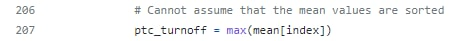
\includegraphics[width=0.7\textwidth,left]{Figures/eotest_turnoff.jpg}
         \caption{Eotest code}
     \end{subfigure}
     \vspace{3mm}
     \begin{subfigure}[b]{\textwidth}
         
         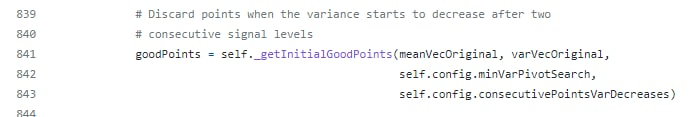
\includegraphics[width=\textwidth,left]{Figures/DMstack_turnoff1.jpg}
     \end{subfigure}    
     \vspace{3mm}
     \begin{subfigure}[b]{\textwidth}
         
         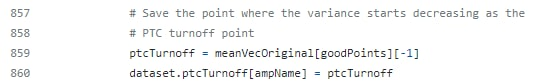
\includegraphics[width=0.85\textwidth,left]{Figures/DMstack_turnoff2.jpg}
         \caption{DM stack code}
     \end{subfigure}
        \caption{Codes used to calculate the PTC-turnoff in \href{https://github.com/lsst-camera-dh/eotest/blob/32c17b0a33b9c099651ed581ee90c1b1101012fb/python/lsst/eotest/sensor/ptcTask.py}{eotest} (a), employed by SLAC, and \href{https://github.com/lsst/cp_pipe/blob/6bae47012f2f119b186509ce7efd963b68b61f0d/python/lsst/cp/pipe/ptc/cpSolvePtcTask.py}{DM stack} (b), the official code for LSST data.}
        \label{fig:Turnoff_codes}
\end{figure}
%%%%%%%%%%%%%%%%%%
Overall, we observed similar behavior for the turn-off of the sensors between our work and SLAC, although the methods used for determination were different, as shown in Figure \ref{fig:Turnoff_codes}. In \textit{eotest}, the PTC-turnoff is defined as the point where the variance is maximum, determined among the data whose residuals are below $5\sigma$. On the other hand, in \textit{DM stack}, the PTC-turnoff is defined as the point where the variance starts to decrease monotonically by at least two points (the number of points to decrease can be modified in the function \_getInitialGoodPoints). According to SLAC, the found FWC was approximately 90000 e$^-$. In our work, however, we found an average turn-off value of $83240$ ADU, which corresponds to an approximate FWC value of $130000 \pm 10000$ e$^-$. \colorbox{red}{(Reference needed for SLAC's FWC value)}

\begin{landscape}
\begin{table}[!htb]
\centering
\caption{Detectors with segments exhibiting low PTC-turnoff values (below 40000 ADU), misclassified PTC-turnoff by the algorithm, bad segments, or discrepancies compared to results obtained by SLAC (parameters highlighted in red). The table presents the detector ID (col1), detector number (col2), vendor (col3), affected segment (col4), PTC parameters (gain, BF effect, and turnoff coefficient; cols 5, 6, 7, and 8, respectively), and detected problem (col9).}
\label{tab:PTC_warnings}
\begin{tabular}{ccccccccp{0.2\textwidth}}
    \hline 
     Detector ID   &   Det Num & Vendor   & Amp   &     Gain &   Read Noise &           $A_{00}$ &   Turnoff & Issue\\
      & & & & $[e^-/$ADU$]$ & $[e^-]$ & & [ADU] & \\
    \hline 
    \hline
    R01\_S00       &              0 & ITL      & C04  &   \textcolor{red}{1.5833} &   6.2061                 &  $\textcolor{red}{-2.0160 \times 10^{-6}}$ & 73461.2   &  SLAC diff \\
    R01\_S00       &              0 & ITL      & C14  &   \textcolor{red}{1.7514} &   6.4150                 &  $\textcolor{red}{-2.1907 \times 10^{-6}}$ & 68032.3   &  SLAC diff \\
    R01\_S20       &              6 & ITL      & C00  &   \textcolor{red}{1.5354} & \textcolor{red}{11.1174} &  $\textcolor{red}{-4.1734 \times 10^{-6}}$ & 65371.7   &  SLAC diff \\
    R01\_S20       &              6 & ITL      & C05  &   \textcolor{red}{1.4837} & \textcolor{red}{15.5104} &  $\textcolor{red}{-4.5175 \times 10^{-6}}$ & 76106.5   &  SLAC diff \\
    R01\_S20       &              6 & ITL      & C06  &   \textcolor{red}{1.5104} & \textcolor{red}{13.5644} &  $\textcolor{red}{-4.3955 \times 10^{-6}}$ & 72293.9   &  SLAC diff \\
    R02\_S20       &             15 & ITL      & C17  &      1.67191              &      5.81973             &  $-2.20396 \times 10^{-6}$                 & 30567.4   & low PTC-turnoff\\
    R03\_S11       &             22 & ITL      & C00  & \textcolor{red}{15.2117}  & \textcolor{red}{44.0087} &  \textcolor{red}{-0.708105}                & 223.072   & SLAC diff - dead?\\
    R10\_S11       &             31 & ITL      & C10  &      1.63413              &      4.13177             &  $-3.65785 \times 10^{-6}$                 & 32842.4   & low PTC-turnoff\\
    R20\_S00       &             72 & ITL      & C17  &      0                    &  \textcolor{red}{0}      & nan                                        &     0     & SLAC diff and dead\\
    R20\_S01       &             73 & ITL      & C00  &      1.6083               &      6.45279             &  $-3.12539 \times 10^{-6}$                 & 35507.4   & low PTC-turnoff\\
    R20\_S12       &             77 & ITL      & C00  &      1.59232              &      4.70427             &  $-8.02249 \times 10^{-6}$                 & 26827.1   & low PTC-turnoff\\
    R30\_S00       &            117 & E2V      & C10  &      0                    &  \textcolor{red}{0}      & nan                                        & 0         & SLAC diff and dead\\
    R41\_S20       &            168 & ITL      & C16  &      1.61074              &      6.07818             &  $-1.98753 \times 10^{-6}$                 & 37863.2   & low PTC-turnoff\\
    R41\_S20       &            168 & ITL      & C17  &      1.59228              &      9.57256             &  $-2.54637 \times 10^{-6}$                 & 26120     & low PTC-turnoff\\
    R41\_S21       &            169 & ITL      & C02  & \textcolor{red}{1.08095}  & \textcolor{red}{62.8775} &  $-4.52943 \times 10^{-6}$                 & 16237.9   & SLAC diff and PTC-turnoff mismatch\\
    R41\_S21       &            169 & ITL      & C11  &      1.61255              &      5.23312             &  $-2.61051 \times 10^{-6}$                 & 32467.3   & PTC-turnoff mismatch\\
    R41\_S21       &            169 & ITL      & C15  &      1.59804              &      5.21757             &  $-2.31531 \times 10^{-6}$                 & 39151.3   & PTC-turnoff mismatch\\
    R41\_S22       &            170 & ITL      & C10  &      1.60171              &      4.76741             &  $-3.2105  \times 10^{-6}$                 & 32369.9   & low PTC-turnoff\\
    R42\_S00       &            171 & ITL      & C17  &      1.6516               &      6.4254              &  $-3.09362 \times 10^{-6}$                 & 30253.3   & low PTC-turnoff\\
    R43\_S10       &            183 & ITL      & C17  &      1.59721              &      8.53352             &  $-2.46596 \times 10^{-6}$                 & 30195.2   & low PTC-turnoff\\
    R43\_S22       &            188 & ITL      & C00  &      1.6348               & \textcolor{red}{5.28826} &  $-4.64678 \times 10^{-6}$                 & 21477.5   & SLAC diff\\
    R43\_S22       &            188 & ITL      & C01  &      1.6348               &      5.28826             &  $-4.64678 \times 10^{-6}$                 & 21477.5   & low PTC-turnoff\\
    R43\_S22       &            188 & ITL      & C02  &      1.55382              &      6.94625             &  $-7.40255 \times 10^{-6}$                 & 30764.3   & low PTC-turnoff\\
    R43\_S22       &            188 & ITL      & C03  &      1.56826              &      7.24918             &  $-4.92713 \times 10^{-6}$                 & 38222.4   & low PTC-turnoff\\
    R43\_S22       &            188 & ITL      & C04  &      1.58147              &      3.76291             &  $-4.88158 \times 10^{-6}$                 & 38143.6   & low PTC-turnoff\\
    \hline
    \end{tabular}
\end{table}
\end{landscape}

\subsection{Gain from Flat Pairs}
Initially, we utilized the PTC method to obtain the gain values. However, this approach can be time-consuming as it requires fitting over a wide range of flux values. Therefore, we explored an alternative method, which we refer to as the \textit{gain by pairs of flats}, that is less time-intensive. The left panel of Figure \ref{fig:Gain_full} displays the gain values for detector 55 in a flux range of $0$ to $\sim 120000$ ADU, including values that exceed the saturation level marked by the vertical lines indicating the PTC-turnoff for each segment. On the right panel, the gain values are slightly further from the saturation level, revealing a bump around $60000$ ADU due to nonlinearity, which will be discussed in Section \ref{subsec:crosstalk_and_linearity}. It is important to note that for the analysis of the gain per pair of flats, we only use data below the PTC-turnoff.
 
\vspace{3mm}
In this section, we highlight the differences we observed between the gain obtained from the PTC and pairs of flats, explore possible ways to reduce these differences, and discuss what can be expected from this alternative method in comparison to the first one.

 \begin{figure}[!htb]
    \centering
    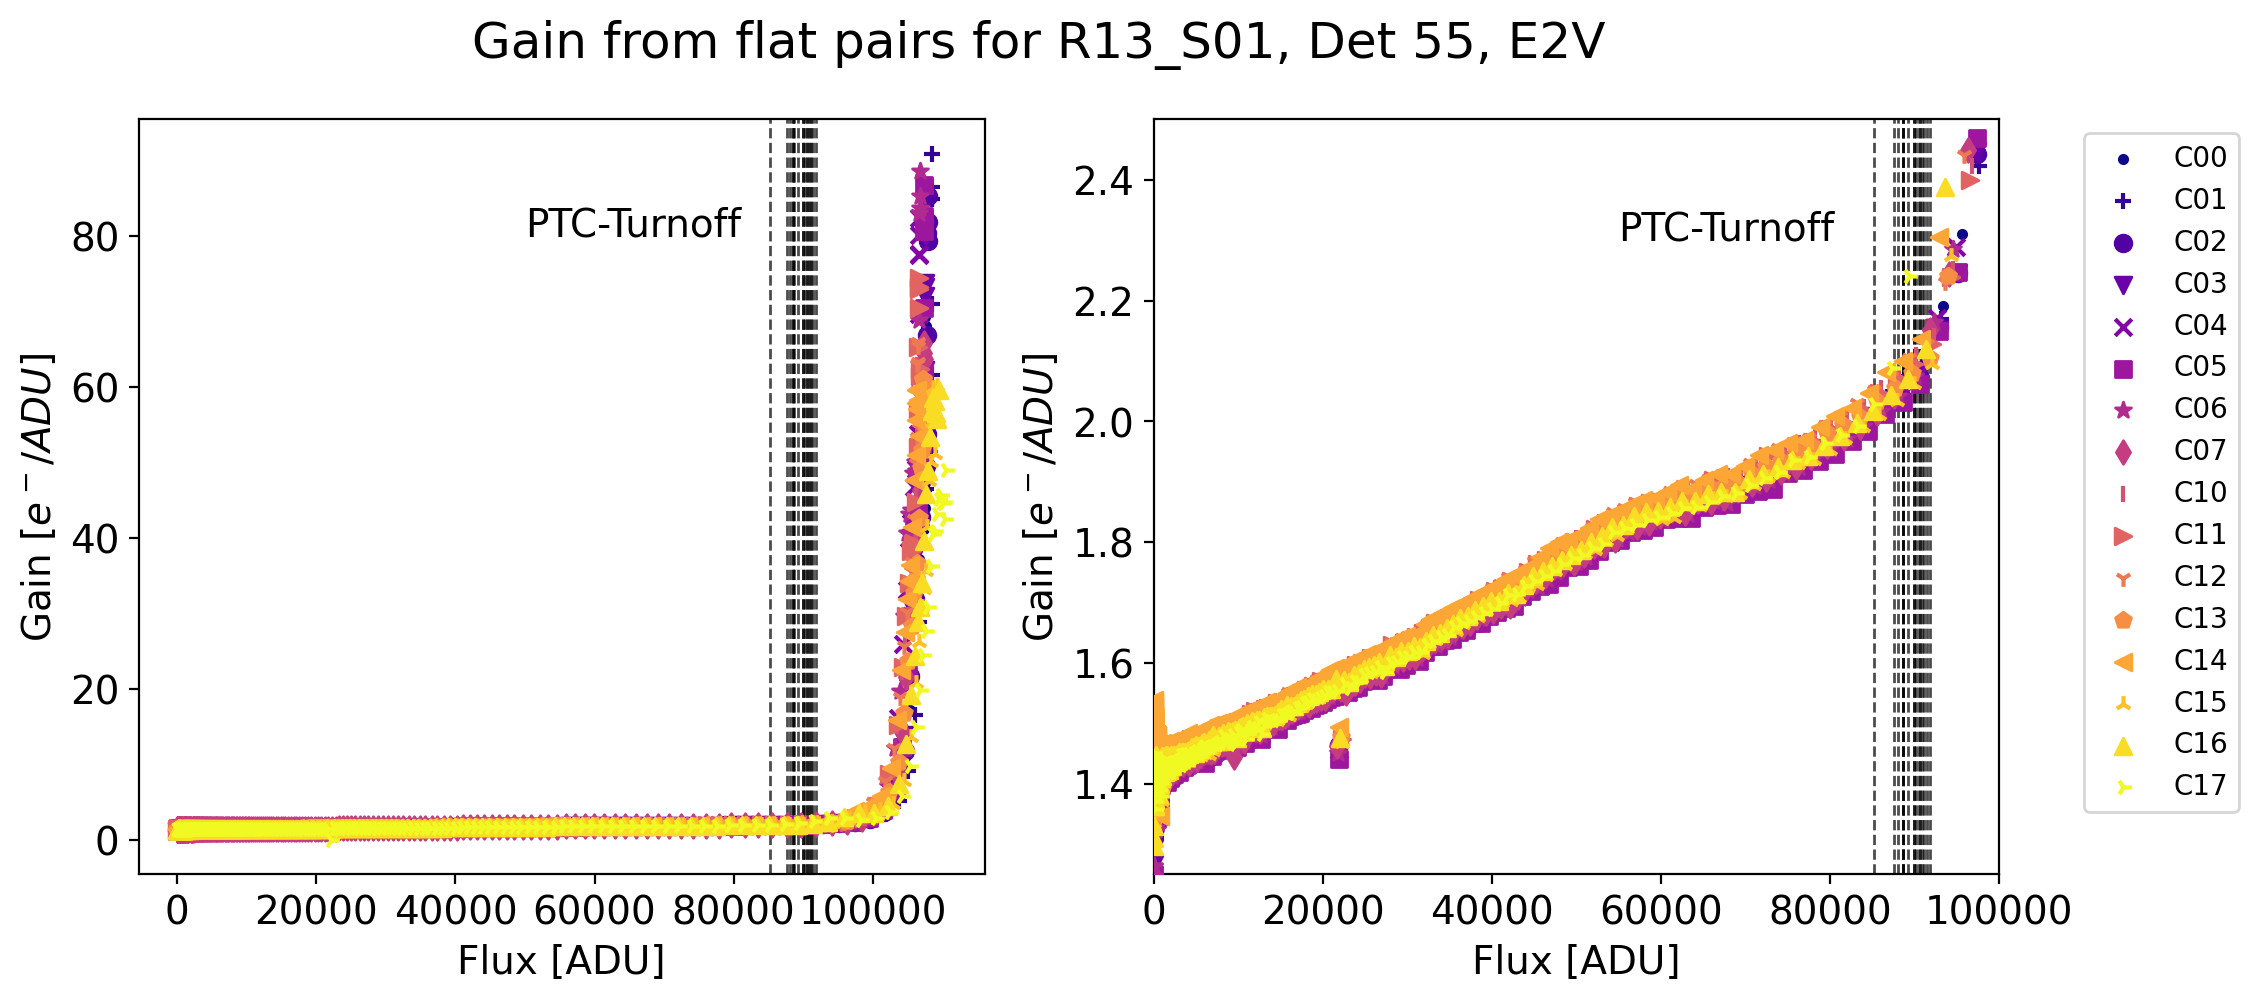
\includegraphics[width=\textwidth]{Figures/Gain_plot_55.png}
    \caption{Gain values obtained from pairs of flat exposures for fluxes up to approximately 120000 ADU for detector 55 (R13\_S01). In both panels, the dashed vertical lines indicate the PTC turnoff values for each of the 16 detector segments, while the colored data points represent the gain as a function of the flux values for each segment. The right panel zooms in on the region up to the PTC-turnoff point shown in the left panel.}
    \label{fig:Gain_full}
\end{figure}

\vspace{3mm}
As mentioned in the methodology (sec. \ref{sec:methods}), we used two code versions (w\_2022\_27 and w\_2022\_32), with the main difference and our focus shown in figure \ref{fig:diff_codes}. This figure illustrates how the two code versions handle statistics to compute gain from pairs of flats. The \textit{w\_2022\_27} version (shown in red) assumes a Gaussian distribution and truncates the distribution to reject outliers, while the \textit{w\_2022\_32} version (shown in green) rejects this assumption. Based on our analysis results described in this section, we recommend using the \textit{w\_2022\_32} version, as the distribution of the operation between two flat images, which is used to calculate the gain, does not follow a Gaussian distribution. Truncating the distribution can alter the expected value for the gain.


\begin{figure}[!htb]
    \centering
    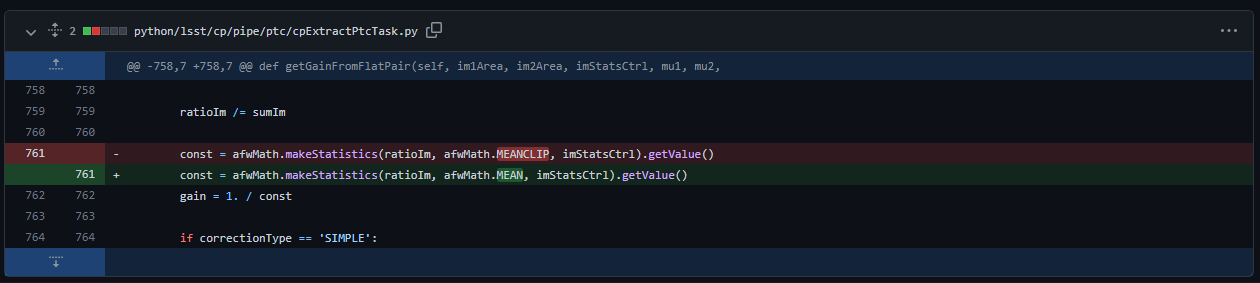
\includegraphics[width=\textwidth]{Figures/Cambio_codigo.png}
    \caption{Difference between the initial code (w\_2022\_27, shown in red) and current code (w\_2022\_32, shown in green) for calculating the gain from a pair of flat fields.}
    \label{fig:diff_codes}
\end{figure}


The version \textit{w\_2022\_27} yielded unexpected results, as shown in figure \ref{fig:relative_error_oldcode}, where the relative percentage error between the gain per PTC and flat pair exceeded 5\% at a flux of 5000 ADU. This was observed for both E2V (upper panel) and ITL (lower panel) detectors. To investigate the cause of this high percentage error, simulations were performed using the methodology described in section \ref{subsubsec:method_Simulation_Gain}.


\subsubsection{Simulation}
Based on the previous result of a 5\% relative error between gains at 5000 ADU, we formulated several hypotheses. Firstly, we considered the possibility that the masks in the flat images could be causing the error, such as if the masks of each image are significantly different and the code uses them for calculations. Secondly, we considered the potential overestimation of read noise. Lastly, we investigated other statistical factors that could be contributing to the error.

\vspace{3mm}
To explore these hypotheses, we conducted simulations using a flat image of a CCD segment and actual segment masks. The use of one mask for both flats, the union of both masks, or different masks for each flat did not account for the observed 5\% error at 5000 ADU, as shown in the top panel of Figure \ref{fig:simulation_masks}. Interestingly, we observed that higher read noise, when using a NONE type correction, resulted in larger discrepancies between the expected and calculated gain (2 $e^-$/ADU). However, subsequent corrections (SIMPLE and FULL), which account for the read noise, accurately calculated the expected gain value. Nevertheless, the bottom panel of the figure, which includes control statistics in addition to the masks, consistently showed a relative percentage error between the gain per PTC and flat pairs above 5\% in all the cases. We further verify this with real data in the next section (\ref{subsubsec:results_gainflats_realdata}).


\begin{figure}[!htb]
     \centering
     \begin{subfigure}[b]{\textwidth}
         \centering
         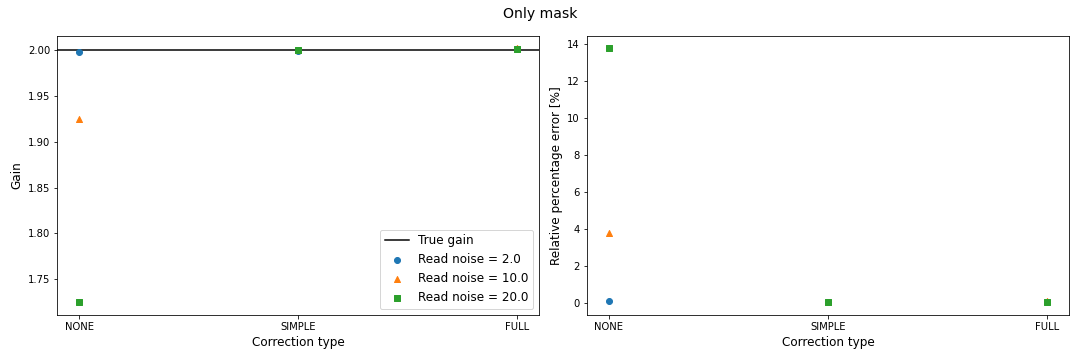
\includegraphics[width=\textwidth]{Figures/Simulation_masks.png}
     \end{subfigure}
     \vspace{3mm}
     \begin{subfigure}[b]{\textwidth}
         \centering
         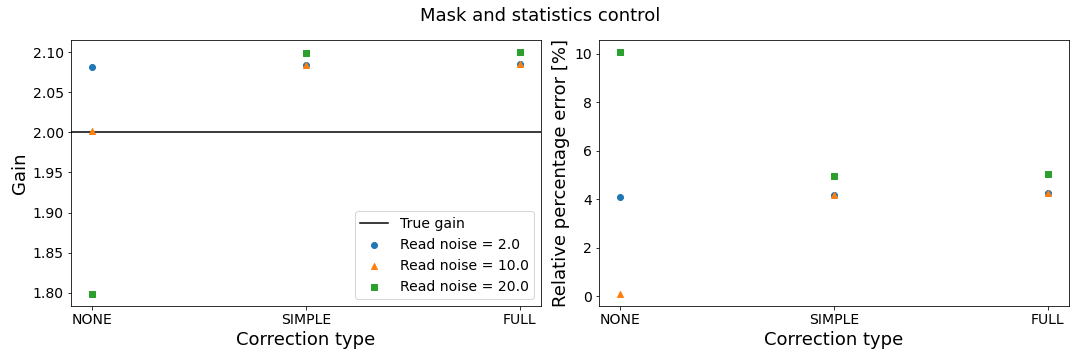
\includegraphics[width=\textwidth]{Figures/Simulation_masks_stats.png}
     \end{subfigure}
        \caption{Simulation results for flat pair gain estimation, shown in the top panel using only masks and in the bottom panel with the addition of control statistics. The average flux value for the simulated flats is approximately $5000$. The left panels display the gain values for three different models, while the right panels show the relative percentage error compared to the expected gain value of 2 $e^-/$ADU. In the left panels, the horizontal black line represents the expected gain value, and the symbols denote various read noise values: blue circles for 2 $e^-/$, orange triangles for 10 $e^-/$, and green squares for 20 $e^-/$. The gain was calculated for three models: NONE, SIMPLE, and FULL, taking these read noise values into account.}
        \label{fig:simulation_masks}
\end{figure}

\subsubsection{Contrasting the simulations with real data} \label{subsubsec:results_gainflats_realdata}

We verified the results obtained from the simulations by comparing them with actual data, specifically for detector 55 (R13\_S01) and all its segments, as shown in figures \ref{fig:GainFlats_NOstats} and \ref{fig:GainFlats_stats}. In these figures, the black crosses represent the gain values obtained from the PTC. The first figure confirms that the use of masks without control statistics results in a relative error of no more than 5\% for any segment of the detector. The highest error observed is 2.25\% at an average flux of 5450 ADU, and the same mask was used for all calculations, i.e., the union of the individual masks. On the other hand, the second figure, which incorporates control statistics along with the masks, reveals that handling the statistics introduces significant discrepancies between the gain values obtained from the PTC and the pairs of flats. In fact, the differences can be as high as 9\% in one of the segments at an average flux of 5450 ADU. These results are consistent with the simulations.
 
 
\begin{figure}[!htb]
    \centering
    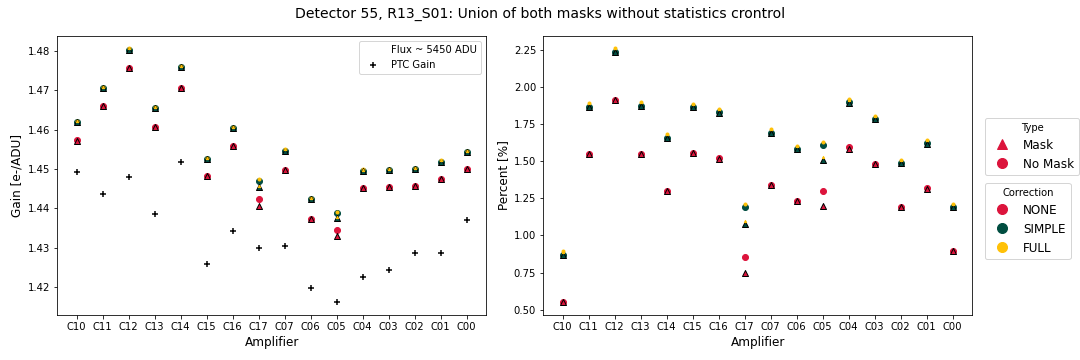
\includegraphics[width=\textwidth]{Figures/GainFlats_NOstats_det55.png}
    \caption{Gain values are shown in the left panel, while the relative percentage error is shown in the right panel, for the 16 segments (amplifiers) of detector 55 (R13\_S01). In the left panel, the black crosses represent the gain values obtained from PTC. The figures in both panels indicate whether the calculation of the gain from flat pairs used masks (triangles) or not (circles), and the colors are associated with the model used to determine the gain: NONE (red), SIMPLE (green), and FULL (yellow). The mask used for calculation was the union of the masks of both flat images per segment, and control statistics were not used.}
    \label{fig:GainFlats_NOstats}
\end{figure}

\begin{figure}[H]
    \centering
    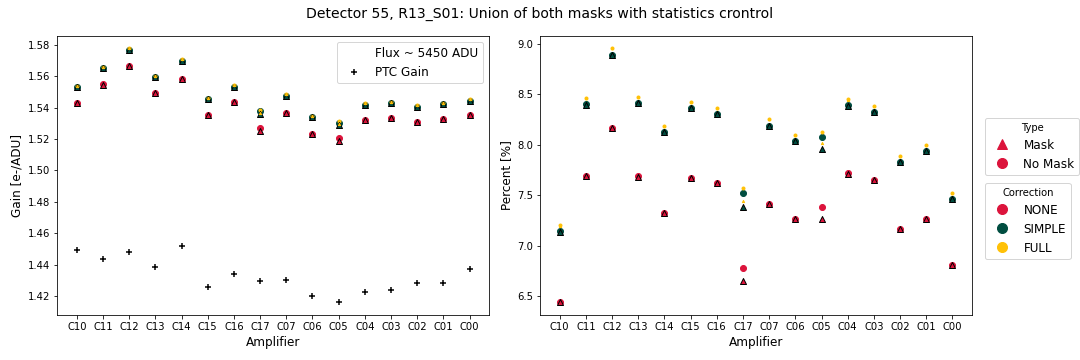
\includegraphics[width=\textwidth]{Figures/GainFlats_stats_det55.png}
    \caption{See description of the figure \ref{fig:GainFlats_NOstats}. This figure used control statistics.}
    \label{fig:GainFlats_stats}
\end{figure}


 Next, we generated plots of the distributions for the operation between the flat images using Equation \ref{eq:ratioIm}, which is the argument of the Lupton equation (Equation \ref{eq:Lupton}) and directly related to the gain. The results are shown in Figure \ref{fig:hist_ratioIM} for each segment of the detector, revealing that the shape of this distribution is not Gaussian. As a result, truncating this distribution can lead to a change in the mean value, which no longer coincides with the mean of the original distribution, resulting in a different gain value than expected.
 
\vspace{3mm}

Subsequently, we constructed the relative percentage error figures for the gain without truncating the distribution, as shown by the green curve in Figure \ref{fig:diff_codes}. The resulting plot is shown in Figure \ref{fig:relative_error}, where the embedded image indicates that for a flux of 5000 ADU, the difference between the two gains is now below 5\%, as confirmed by the simulations. Using this result, we estimated a general relationship for the gain, taking into account the distributions of the linear fit parameters, as shown in Figure \ref{fig:histogram_linearfit}. The linear fit was performed between 5000 and 10000 ADU. In the top left panel of this figure, we can see the distribution of slopes by vendor, revealing a clear bimodality, with E2V detectors having a slightly higher slope compared to ITL, with mean values of $(0.00046 \pm 0.00004)$ and $(0.00027 \pm 0.00004)$ \% ADU, respectively. In the bottom panel of this figure, we have the intercept with the $y$-axis (i.e., the percentage error axis between the gains), which shows an overall mean across the detectors with no appreciable distinction by vendor, having a value of $(-0.5 \pm 0.5)$ \%. Thus, the relative percentage error between 5000 and 10000 ADU for each vendor is given by:

\begin{itemize}
    \item E2V: $Error_{2Gain} = (0.00046 \pm 0.00004) F - (0.5 \pm 0.5)$, where the error interval is ($1.8 \pm 0.7$, $4.1 \pm 0.9$) \%.
    \item ITL: $Error_{2Gain} = (0.00027 \pm 0.00004) F - (0.5 \pm 0.5)$, where the error interval is ($0.85 \pm 0.7$, $2.2 \pm 0.9$) \%.
\end{itemize}
 
\begin{figure}[!htb]
    \centering
    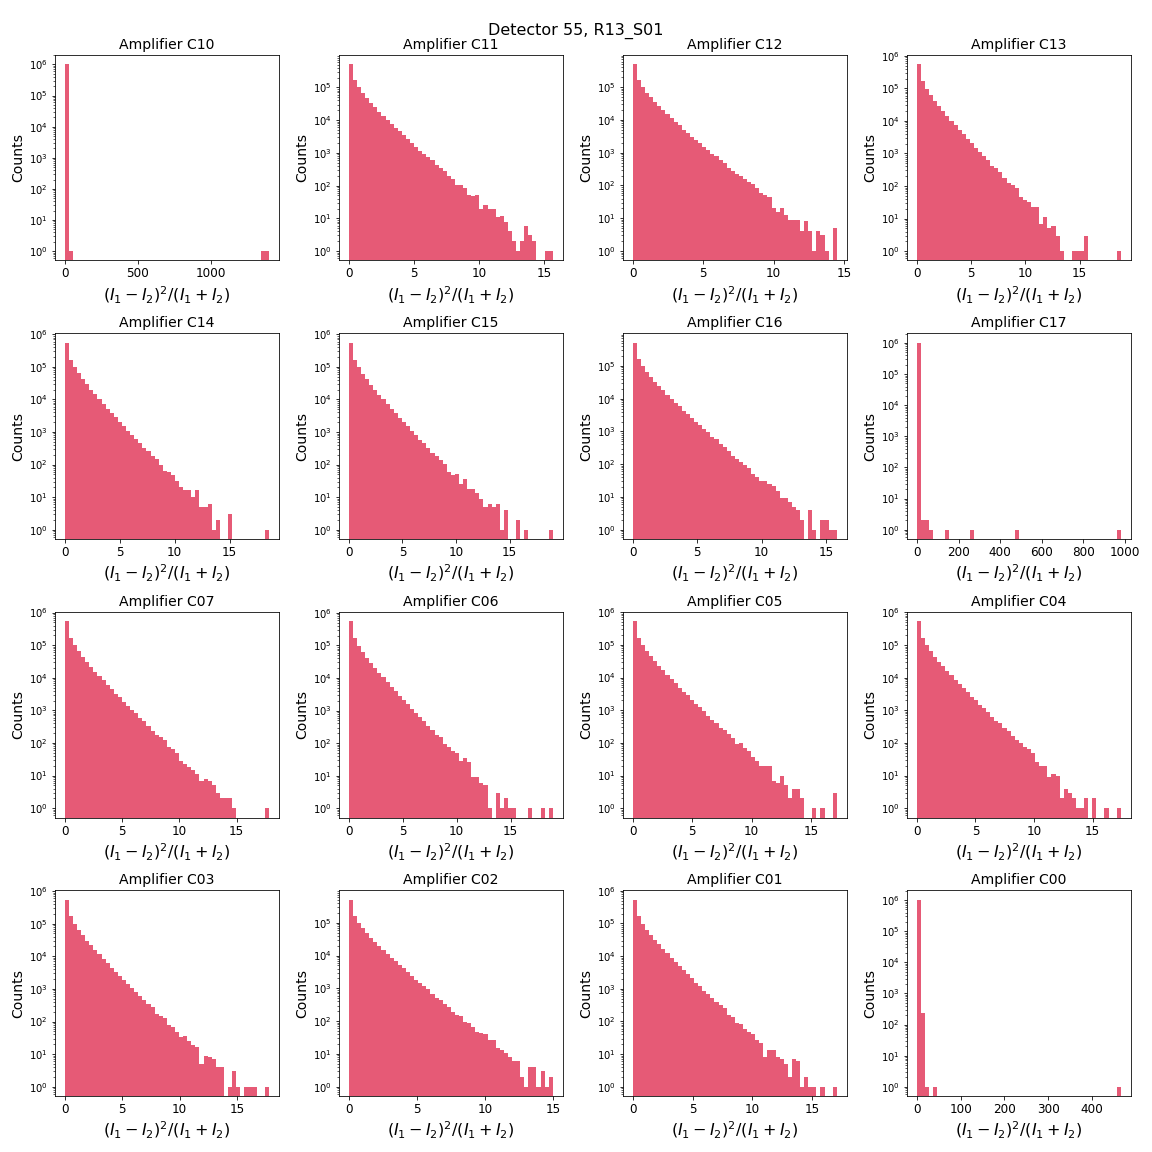
\includegraphics[width=\textwidth]{Figures/Histogram_ratioIM_det55.png}
    \caption{Histogram of the distribution for $\frac{(I_1 - I_2)^2}{I_1 + I_2}$ for each segment of detector 55 (R13\_S01). }
    \label{fig:hist_ratioIM}
\end{figure}


\begin{figure}[!htb]
     \centering
     \begin{subfigure}[b]{\textwidth}
         \centering
         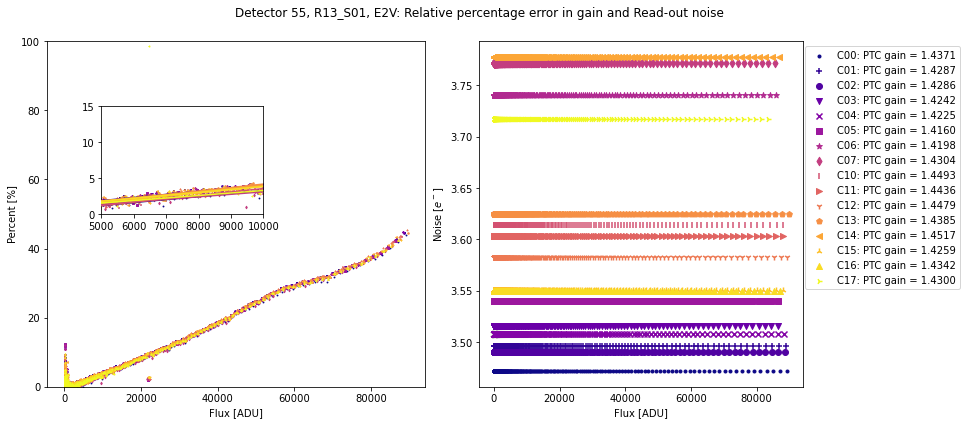
\includegraphics[width=\textwidth]{Figures/Relative_Error_Gain_Noise_detectorR13_S01.png}
     \end{subfigure}
     \vspace{3mm}
     \begin{subfigure}[b]{\textwidth}
         \centering
         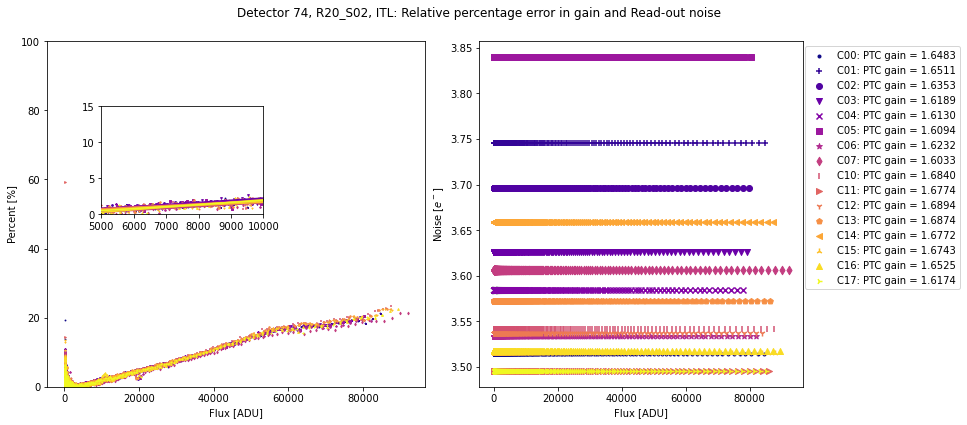
\includegraphics[width=\textwidth]{Figures/Relative_Error_Gain_Noise_detectorR20_S02.png}
     \end{subfigure}
        \caption{Refer to the description of the figure \ref{fig:relative_error_oldcode}. This plot showcases the improved version of the code (version w\_2022\_32) that no longer utilizes a clipped mean}
        \label{fig:relative_error}
\end{figure}

\begin{figure}[!htb]
     \centering
     \begin{subfigure}[b]{\textwidth}
         \centering
         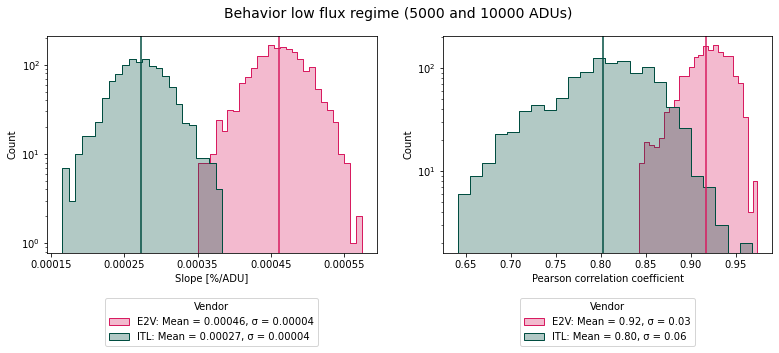
\includegraphics[width=\textwidth]{Figures/Histogram_slope_corr_new.png}
     \end{subfigure}
     \vspace{3mm}
     \begin{subfigure}[b]{\textwidth}
         \centering
         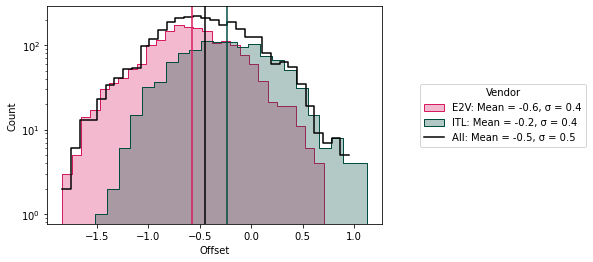
\includegraphics[width=0.7\textwidth]{Figures/Histogram_offset_new.png}
     \end{subfigure}
        \caption{Histograms of the slope (top left), Pearson's correlation coefficient (top right), and $y$-axis intercept (offset, bottom panel) for the linear fit performed in the flow region between 5000 and 10000 ADU for the gain. The construction of these histograms utilized the updated code (version w\_2022\_32), and the vendor is indicated by the colors, with E2V in red and ITL in blue. The vertical lines represent the mean value for each case.}
        \label{fig:histogram_linearfit}
\end{figure}


\subsection{Crosstalk and Nonlinearity Correction} \label{subsec:crosstalk_and_linearity}

As part of our final analyses during this internship, we quantified and assessed whether the crosstalk effect and nonlinearity impact the shape of the PTC and/or the fundamental parameters such as gain, read noise, BF effect, and turnoff coefficient.

\vspace{3mm}

As described in Section \ref{subsec:method_Crosstalk}, we had access to the crosstalk matrices for detector 32 (ITL) and 139 (E2V), which are shown in Figure \ref{fig:crosstalk_matrix}. Applying the methodology of that section, we found that the differences between PTCs with and without crosstalk correction are negligible, as shown in Figure \ref{fig:crosstalk_corr32} and Figure \ref{fig:crosstalk_corr139}. These figures illustrate that the variance differences are consistently below 0.1 ADU when considering the region below saturation. In contrast, the most significant variance in the parameters is approximately $\sim 0.1$\% for read noise and BF effect coefficient, and approximately $\sim 0.07$ \% for gain and turnoff. The most significant differences were found in the ITL detector segments. Based on these findings, we conclude that crosstalk does not have a considerable effect on the parameters, and correcting this effect is unnecessary, as it does not alter the shape of the PTC.


\begin{figure}[!htb]
    \centering
    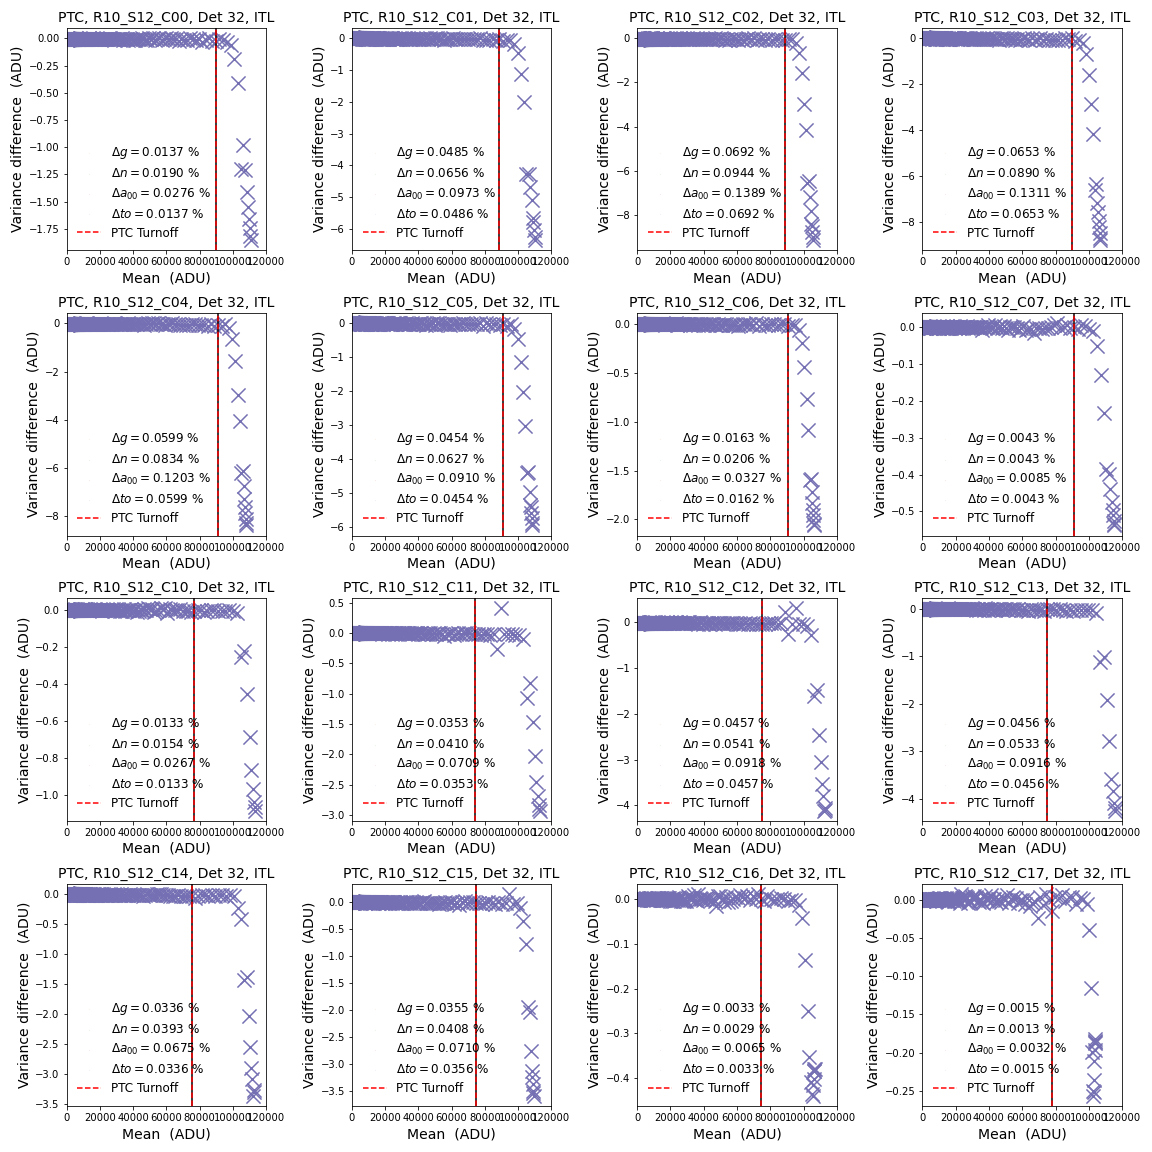
\includegraphics[width=\textwidth]{Figures/ptc_crosstalk32.png}
    \caption{The plot displays the variance difference versus the mean for detector 32 (R10\_S12) from vendor ITL, with the variance difference calculated between the variance values without and with crosstalk correction. Each CCD segment is shown, with vertical lines indicating the PTC-turnoff values. The legends show the parameter differences: $\Delta g$ for gain, $\Delta n$ for read noise, $\Delta a_{00}$ for the BF effect coefficient, and $\Delta to$ for the PTC-turnoff.}
    \label{fig:crosstalk_corr32}
\end{figure}

\begin{figure}[!htb]
    \centering
    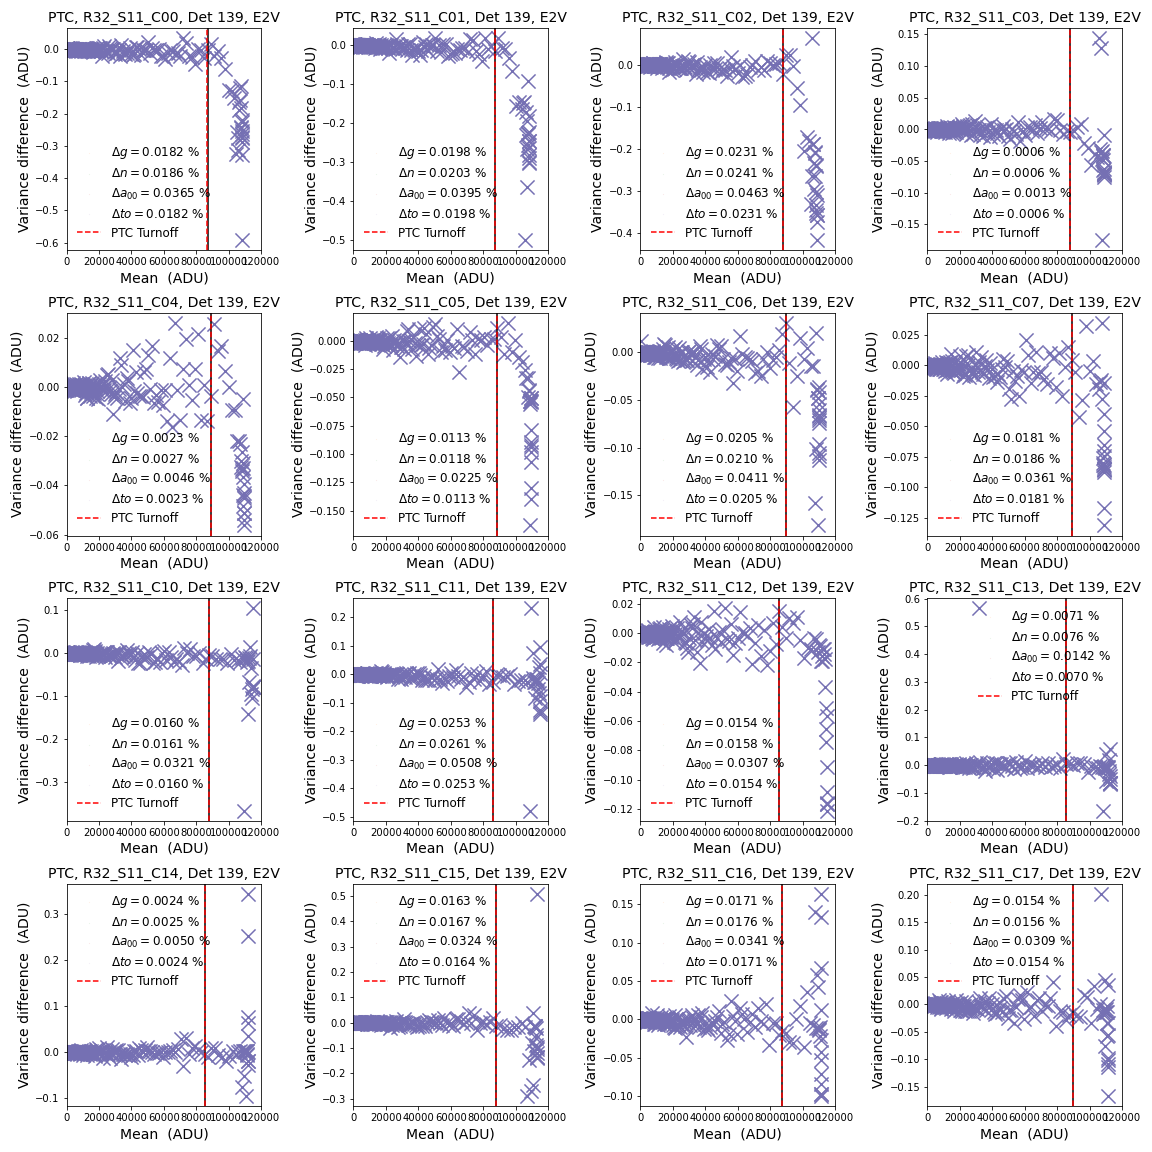
\includegraphics[width=\textwidth]{Figures/ptc_crosstalk139.png}
    \caption{Refer to the description of the figure \ref{fig:crosstalk_corr32}. This plot is for detector 139 (R32\_S11) for vendor E2V.}
    \label{fig:crosstalk_corr139}
\end{figure}

Finally, to verify the impact of the 12-node cubic spline linearizer on the PTC shape, we applied it to the data. The results of correcting only for crosstalk (orange dots), only for nonlinearity (blue diamonds), correcting for both effects (gray triangles), and using uncorrected data (magenta squares) are presented in Figure \ref{fig:varmean_crosstalk}. We observe that the uncorrected data show a bump around 60000 ADU, while the crosstalk-corrected data consistently align with the uncorrected data (also showing the bump), and the data corrected for nonlinearity flatten it. This suggests that making corrections for nonlinearity alone has a more significant impact on the data than making both crosstalk and nonlinearity corrections. Once again, we conclude that crosstalk correction is not necessary as it does not affect the shape or parameters of the PTC.


\begin{figure}[!htb]
     \centering
     \begin{subfigure}[b]{0.49\textwidth}
         \centering
         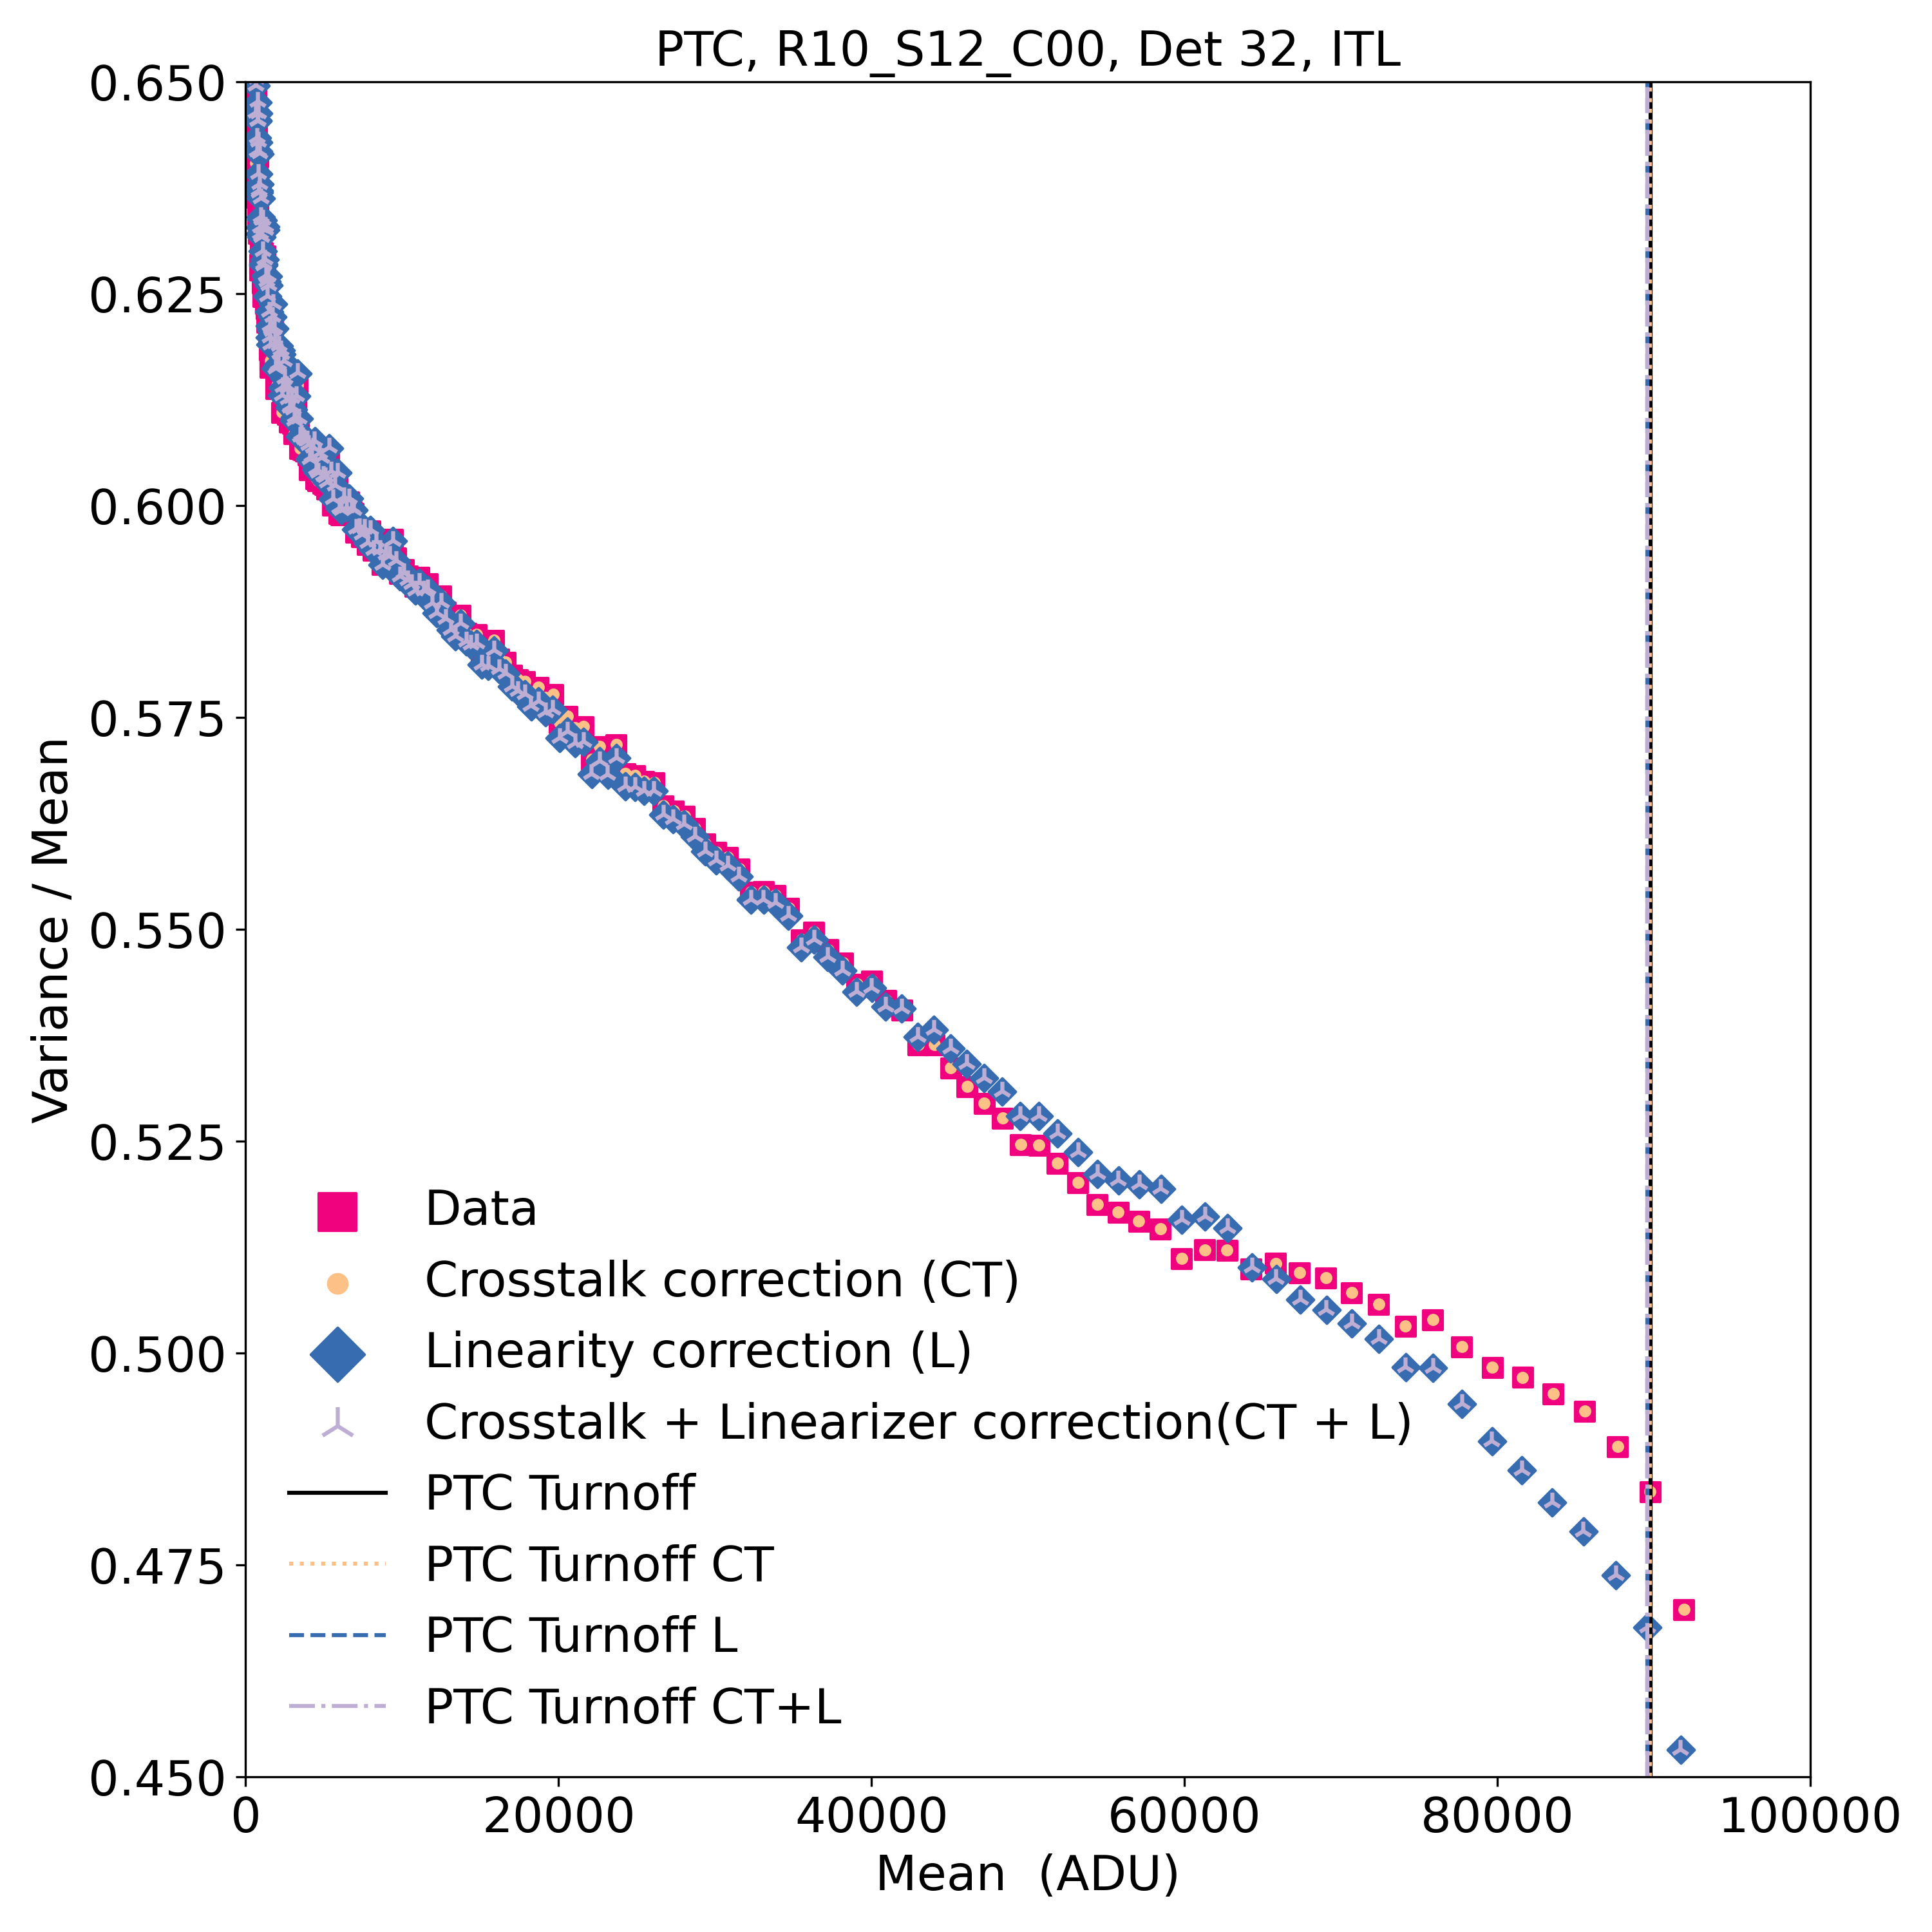
\includegraphics[width=\textwidth]{Figures/Variance_Mean_vs_Mean32.png}
     \end{subfigure}
     \hfill
     \begin{subfigure}[b]{0.49\textwidth}
         \centering
         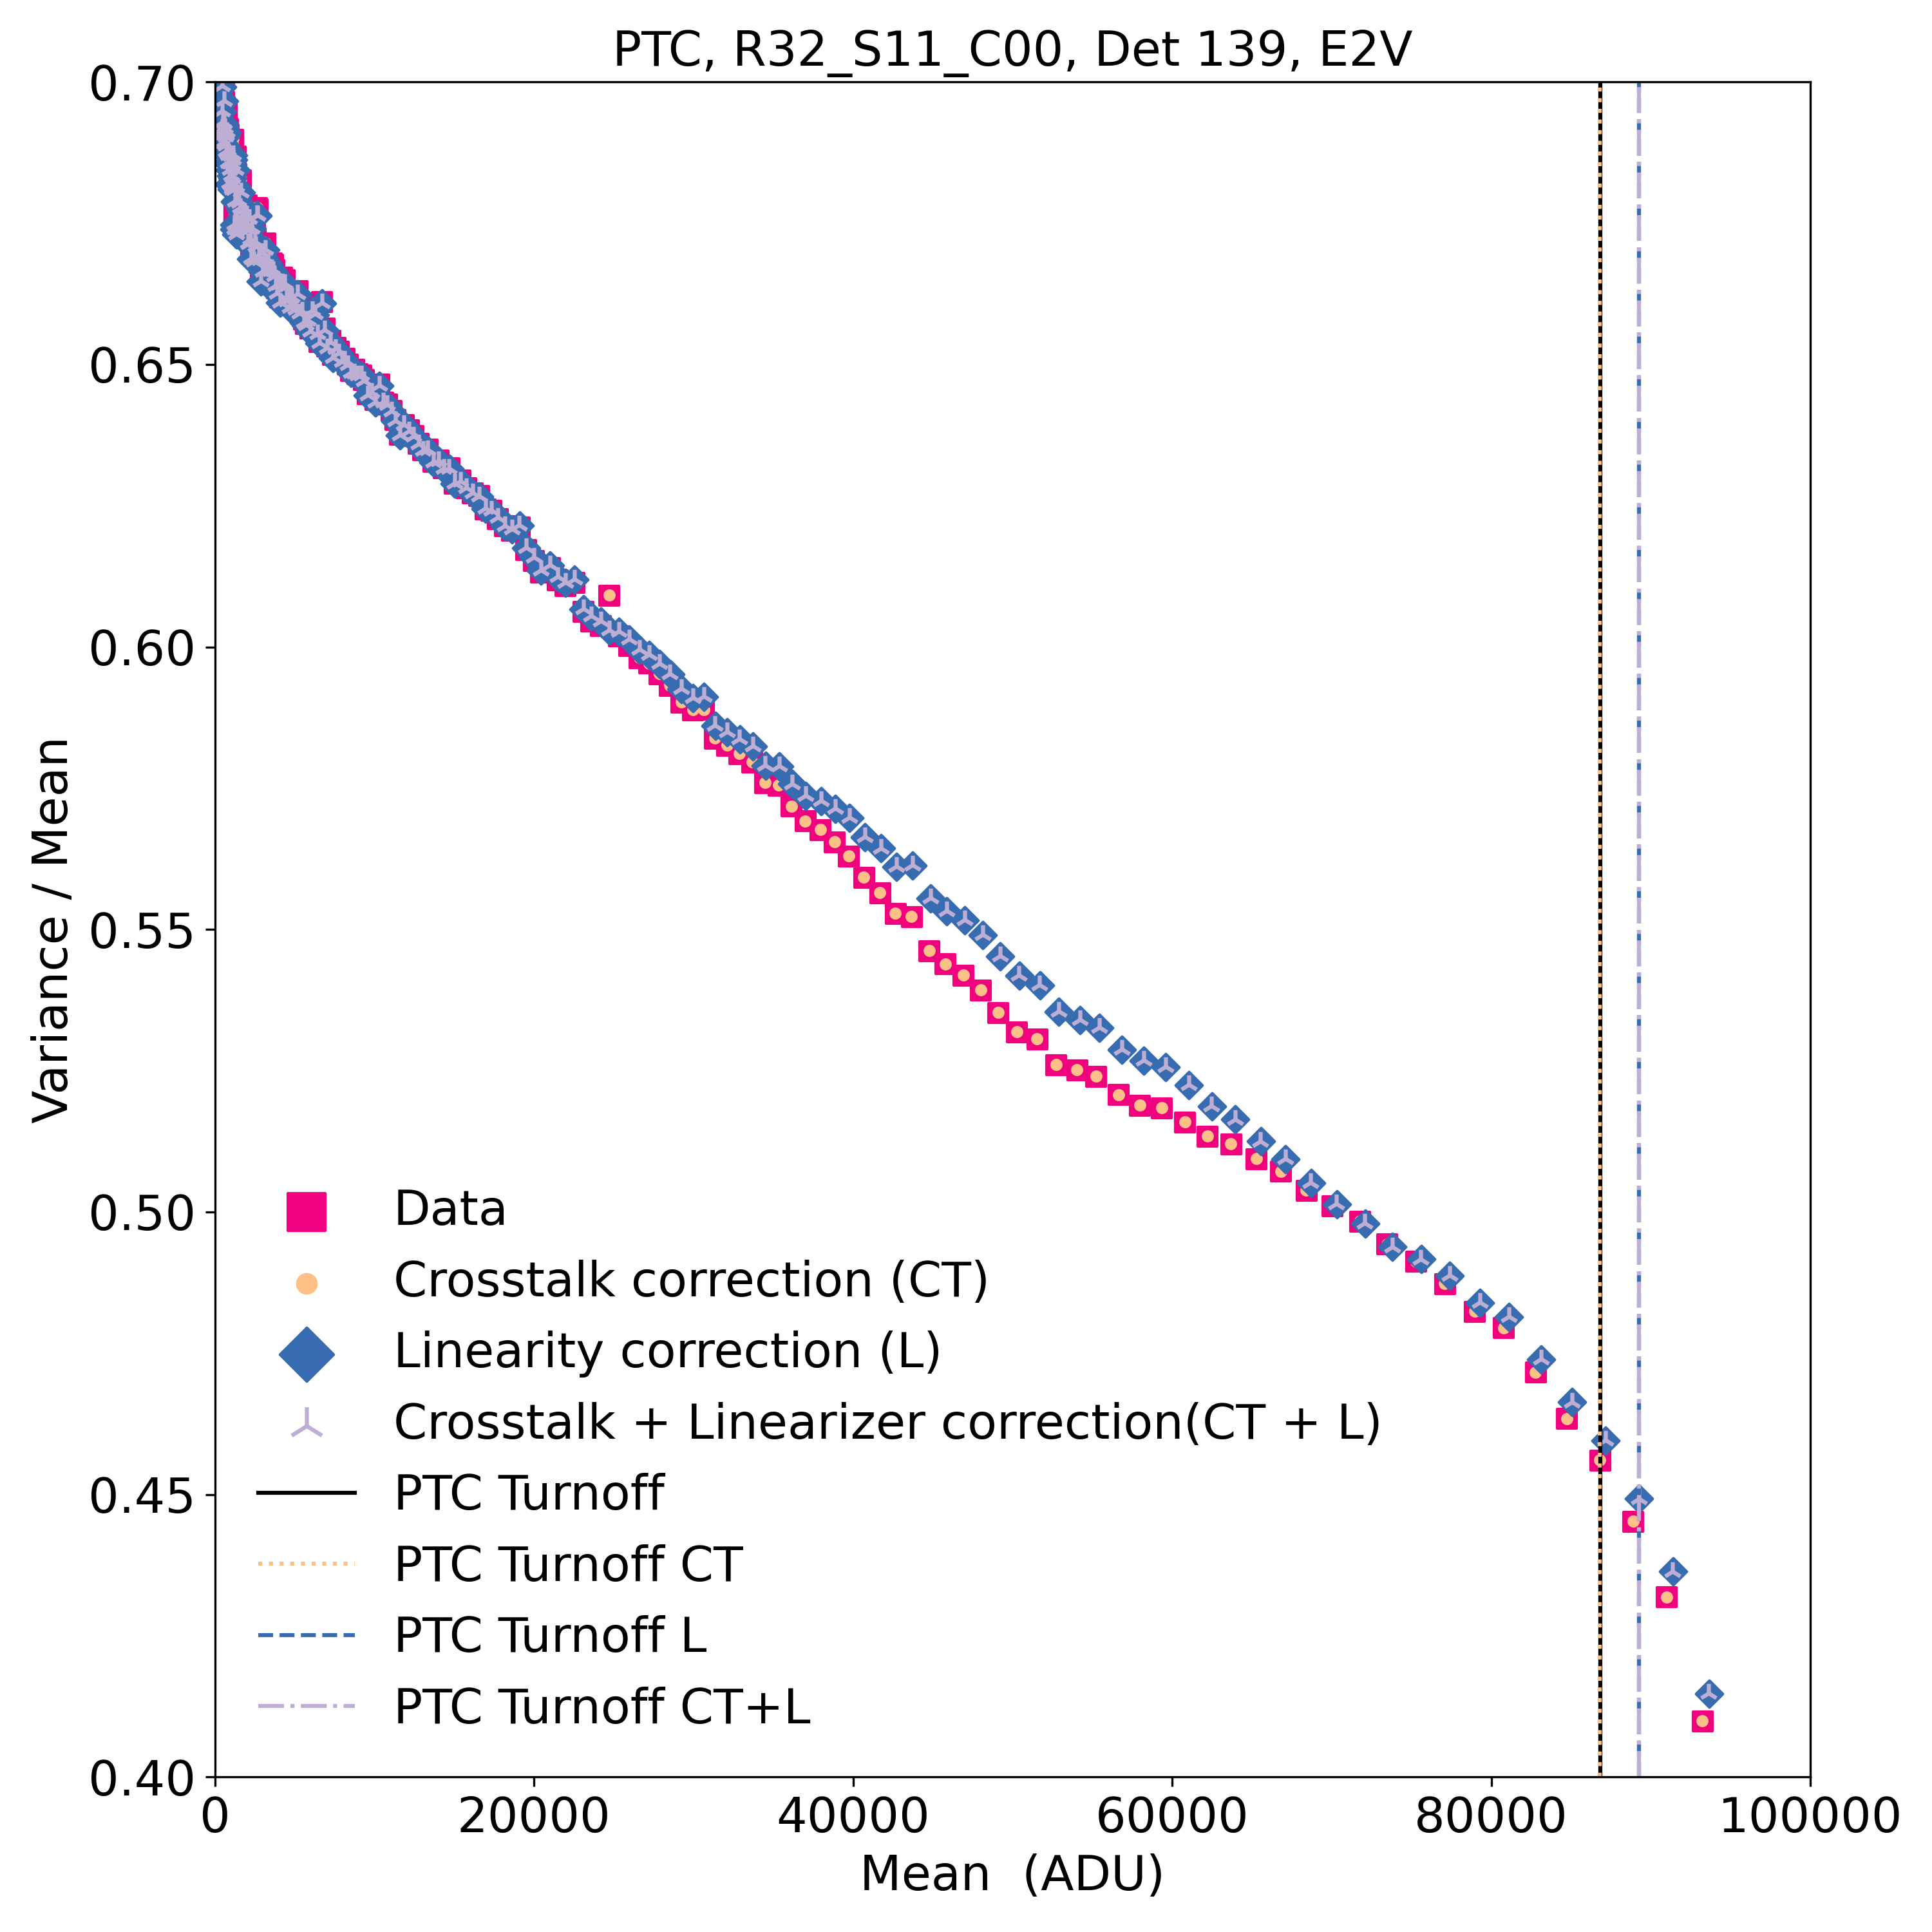
\includegraphics[width=\textwidth]{Figures/Variance_Mean_vs_Mean139.png}
     \end{subfigure}
        \caption{Variance normalized by mean vs. mean for detector 32 (R10\_S12) for vendor ITL (left) and detector 139 (R32\_S11) for vendor E2V (right). Data with no correction for crosstalk and nonlinearity is shown in magenta squares. Data corrected for crosstalk is shown with orange dots, while data corrected for nonlinearity is shown with blue diamonds. Triangles represent data with corrections for both crosstalk and nonlinearity. Vertical lines indicate the location of the turnoff.}
        \label{fig:varmean_crosstalk}
\end{figure}
%\section{Conclusions} \label{sec:conclusions}

We present in this report a list of the sensors that present differences in the parameters with those obtained by SLAC, a PTC with low turnoff, and an inadequate classification of the same so that they can be reviewed later. We use the default value to determine the turnoff via \textit{DM stack}: decrease by at least 2 points to indicate shutdown.

\vspace{3mm}

We find in the PTC study that there is a bimodality per vendor for gain and $a_{00}$ and a more generalized behavior for read noise and turnoff. The average value we found for the gain in the E2V sensors of $1.49 \pm 0.05$ and $1.69 \pm 0.05$ $e^{-}/ADU$ for ITL. The coefficient of the BF effect has an average value of $(-3.0 \pm 0.1)\times 10 ^{-6}$ and $(-1.7 \pm 0.2)\times 10 ^{-6}$ for E2V and ITL, respectively. In addition, ITL detectors present a higher read noise dispersion compared to E2V ($6.7 \pm 1.0 \; e^{-}$ and $5.4 \pm 0.2 \; e^{-}$, respectively). The results obtained in this work are generally congruent with those obtained by SLAC. However, the main difference was observed in the Full Well Capacity value: in this work, we found a value of $130000 \pm 10000$ e$^-$, while SLAC a value of $90000$ e$^-$, which is a product of the different ways of calculating the turnoff between \textit{eotest} and \textit{DM stack}.

\vspace{3mm}

The analysis between the gain obtained from a pair of flats and the gain obtained from the PTC initially yielded a relative percentage error for low fluxes (5K and 10K ADU) higher than 5\%. This result led to a thorough investigation of its origin, finding that the distribution following the Lupton equation for flat images is not of Gaussian type, so the truncation of the distribution to calculate the statistics generating a shift of the mean value, and consequently, larger values of gain concerning the PTC gain. Therefore, this calculation was performed without truncation and obtained percentage differences between these two gains of $(1.8 \pm 0.7, 4.1 \pm 0.9)$ for E2V and $(0.85 \pm 0.7, 2.2 \pm 0.9)$ for ITL, where these intervals correspond to a flow region between 5000 and 10000 ADU. Consequently, the respective report was made and finally implemented in the main code. 


\vspace{3mm}

Finally, the linearity correction fixes the observed bump around 50K-60K ADU. Whereas performing a correction for crosstalk does not affect the shape of the PTC, nor does it significantly modify the parameters. Therefore, we recommend correcting for linearity only.  


%\section{Acknowledgments} \label{sec:acknowledgments}


I would like to express my sincere gratitude to the entire RECA internship program team for their vision and efforts in creating this program that has provided an invaluable opportunity for research and learning for students in Colombia. I am also grateful to LSSST Corporation for generously supporting the realization of this project.

I am deeply thankful to my advisors, Drs. Andrés M. Plazas and Craig Lage, for their guidance, mentorship, and unwavering support throughout this learning journey. Their expertise, patience, and willingness to address my questions have been instrumental in shaping the outcomes of this project. Despite the challenges of virtual collaboration, their dedication and mentorship have fostered a close relationship that I deeply appreciate.

I would also like to acknowledge my colleague Jerónimo Calderón for the engaging discussions, valuable feedback, and camaraderie during the course of this project.

Finally, I am grateful to all other individuals, including fellow researchers and collaborators, who have provided assistance, advice, and encouragement during this project. Your support has been invaluable in the completion of this work.


\appendix
% Include all the relevant bib files.
% https://lsst-texmf.lsst.io/lsstdoc.html#bibliographies
\section{References} \label{sec:bib}
\renewcommand{\refname}{} % Suppress default Bibliography section
\bibliography{local,lsst,lsst-dm,refs_ads,refs,books}

% Make sure lsst-texmf/bin/generateAcronyms.py is in your path
\section{Acronyms} \label{sec:acronyms}
\addtocounter{table}{-1}
\begin{longtable}{p{0.145\textwidth}p{0.8\textwidth}}\hline
\textbf{Acronym} & \textbf{Description}  \\\hline

DM & Data Management \\\hline
CCD & Charge-Coupled Device
\end{longtable}

% If you want glossary uncomment below -- comment out the two lines above
%\printglossaries





\end{document}